\section{The problem of fakes}

The reconstructed objects (leptons, photons, $b$-jets, etc.) in a collision event are used to perform a wide range of SM measurements 
or searches for evidence of BSM physics. The assumption is that these objects are `real` representing the desired particles 
in the final state used in the analysis. 
In practice, the reconstructed objects might not be always `real`. In fact, they may be something completely different that
was mistakenly reconstructed as the desired object, called `fake`. 
For the purpose of the analysis presented in this thesis, the focus is on `fake` leptons. 
To illustrate the problem, a hadronic jet may deposit more energy in the electromagnetic calorimeter than the hadronic calorimeter, 
or that it leaves a narrow deposit of energy leading the reconstruction alogorithms to mistake this jet for an electron.
From the analysis point of view, the `fake` electron will pass all the selection criteria and will be indistinguishable from 
a `real` electron. 
It is important for the analysis that requires a reconstructed electron to model the fake electron background to get a sound 
result. This example was given with electrons, but can be generalized to muons as well. 
In short, any analysis that uses leptons in the final state must account for the `fake` lepton background. 
This background can be more or less important depending on the detector, the analysis selection, and the number of leptons required. 
To estimate this background it is important to first understand what type of processes lead to fake leptons.


\section{Common processes for faking leptons}

The reconstruction of `fake` leptons can be an instrumental effect related to the inability to identify the object based on 
its measured properties by the detector. In this case, the reconstructed lepton is not a real lepton and the production process 
will be different for electrons and muons.

The reconstruction of electrons relies on the observation of well aligned particle hits in the layers of the ID that are consistent 
with an energy deposition in the EM calorimeter. Photons can mimick this signature since they deposit energy in the EM 
calorimeter that happens to be alligned with a charged track. A jet for example containing charged and neutral pions can 
lead to such scenarios. It is possible for the jet to have one charged pion leaving a track similar to that of an electron.
The decay of $\pi^0$ mesons to photons in this jet can deposit energy in the EM calorimeter leading to the required signature.
Another mechanism that can lead to fake electrons is the emission of photons via Brehmstrahlung from high energy muons. 
The muon track can be mistaken for that of an electron and the photons interact with the EM calorimeter leading to a
signature similar to that of electrons. An additional process is that of photon conversions into a $e^+e^-$.

The reconstruction of muons relies on the observation of tracks from the ID matched to tracks from the muon spectrometer.
It is possible for charged hadrons with long lifetime to traverse the calorimeter layers and leave hits in the muon spectrometer.
These hits may coincide with other hits from the ID due to the random activity in the event. As a result, a muon can get
reconstructed. Another instance may occur when pions or kaons decay in-flight to muons in the muon spectrometer
and happen to align with the primary vertex.

The leptons that are used in the physics analyses must be coming from the hard scatter, generally referred to as prompt leptons.
There is another case where the reconstructed lepton is a real lepton but is not a lepton coming from the hard interaction,
referred to as non-prompt leptons. Non-prompt leptons can be produced from heavy flavor meson decays with a low energy activity 
around the lepton which allows it to pass isolation requirements. A good example of this type of process is the 
semi-leptonic decay of top quark pair which contribute to final states with two leptons. 

For the rest of the thesis, the fake leptons will be referred to as fake/non-prompt (FNP) leptons.
There are several methods used to perform the estimation of FNP lepton backgrounds. 
A method that the author developed will be described next along with a standard method for estimating this type of backgrounds.
The benefit of having two methods for estimating the FNP lepton background is to have enough confidence in the final estimate. 
The two methods use different assumptions which naturally leads to a more robust estimation of this difficult background.
Moreover, the final estimate of the FNP lepton background is taken as a statistical combination of the estimates from the 
two methods leading to a reduction of the systematic uncertainties on the estimate.


\section{Monte Carlo Template Method}
\graphicspath{{figures/mct/}}

\subsection{Motivation}
The processes leading to FNP leptons depend on the selection applied in the analysis. For instance, a selection with same-sign leptons 
will have contributions from top quark pair production (\ttbar) or the associated production of a vector boson and jets 
($W$+jets or $Z$+jets).%, or opposite sign $W$ pair production ($W^+W^-$). 
These processes cannot give two leptons of the same electric charge unless there is a charge mis-measurement (mainly affecting electrons) 
or that a FNP lepton was produced. It is possible to generate the processes that can contribute to a FNP lepton, such as \ttbar or 
$V$+jets, with Monte Carlo event generators processed through Geant4 detector simulation of the ATLAS detector.  
This approach will yield an estimate however it might not be reliable. For instance, the detector simulation itself might not 
reproduce the true behavior of the interaction of the physics objects with the detector, particularly when looking at rare processes 
such as the production of FNP leptons. The second limitation is in the generation of enough MC events to probe the region of the 
phase space targetted by the analysis which affects the statistical uncertainties in the estimates.
The latter concern is addressed by ensuring that the simulations for the major backgrounds (\ttbar and $V$+jets) have much 
higher event count than the corresponding number of events observed in the data sample.
In fact, these backgrounds have a large number of simulated events because they are important for many analyses 
(including SM measurements and BSM searches).
The rest of the section will concentrate on addressing the former limitation. 

%% ****
%% low statistics of the tri-lepton samples and the variety of sources of fake leptons.
%% It is difficult to rely on data-driven (including ME-based) methods that rely on inverting the isolation requirement given we deal with multi-jet final states. Inversion of the isolation requirement produces a sample with much more energetic jets than in the sample with the un-inverted isolation. 

%% ''
%% picked variables that offer good separation between processed with prompt and ``fake'' leptons.
%% It is nice that the corrections are close to one but they do not have to be. For example, their deviations from unity depend on the decay modes of heavy flavor hadrons that are implemented in simulations.

%% Is the showering of the samples used to measure the correction of the fake rate and the that of the samples it is applied to the same? if not, is there a potential systematic difference that has to be taken into account?

%% We used Herwig for showering of all the samples that require corrections to the fake rates.



\subsection{Description of the method}

The MC template method relies on the correct modelling of FNP leptons kinematics in 
MC simulation to extrapolate background predictions from control regions to the signal regions.
The method assumes that the kinematic shapes for each source of FNP lepton is correctly modeled in the simulations, 
and the normalization for each source is extracted in a combined fit to data control regions.
The number of normalization factors depend on the number of identified origins of the FNP lepton in the signal regions
and the control regions are designed to constrain these factors in regions enriched with FNP leptons from the same origin.

To illustrate the approach, we describe the application of the method in SS/3L analysis later described in this thesis.
The processes of interest that may lead to a FNP lepton or a charge flip are $\ttbar$ and $V$+jets. 
FNP leptons are classified using an algorithm that navigates the generator particle record to determine where the FNP lepton 
is originating from. 
The lepton is classified as either an electron or a muon that is prompt from decays of on-shell $W$ and $Z$ bosons, 
non-prompt from a heavy flavor $b$ decay (HF), or fake from mis-identification of a light flavor jet or a photon (LF). 
In the case of an electron, we further classify the prompt electrons to prompt electrons with the correct charge or with a 
charge mis-measurement, commonly named charge flip.
In total, five categories referred to as MC templates are construced following the classification illustarted 
in figure~\ref{Fig:fakes_classification}.

\begin{figure}[t!]
\centering
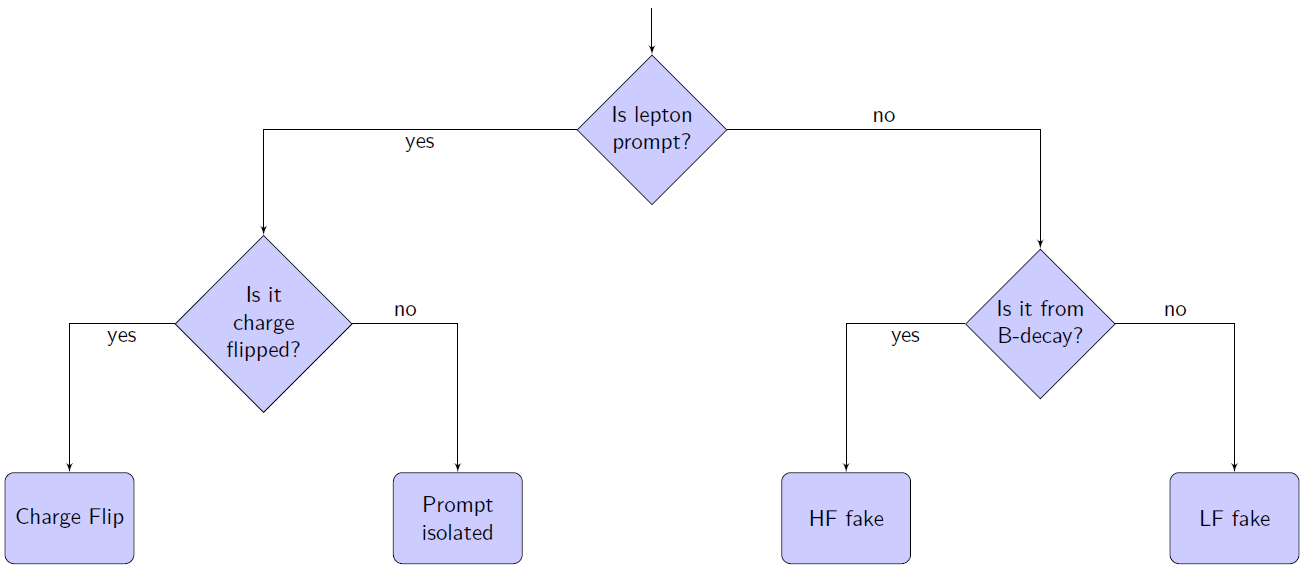
\includegraphics[width=0.7\textwidth]{MC-tmpl}
\caption
{Lepton classification.
}
\label{Fig:fakes_classification}
\end{figure}

\subsection{Correction factors}

The FNP estimate relies on kinematic extrapolation using processes expected to contribute via FNP leptons from control regions 
with low jet multiplicity and \met, to the signal regions that require high jet multiplicity and \met. 
The control regions are chosen to separate FNP leptons from HF origins and FNP leptons from LF origins.
For instance, a control sample characterized by the presence of a $b$-jet will be enriched in processes with one FNP lepton that is 
coming from a HF decay, while a sample characterized by the absence of a $b$-jet will have one FNP lepton from LF decay.
The presence of one FNP lepton in the control sample allows the correction of the production rate of these FNP leptons 
by performing a fit to data. 

For example, if a Z$\to\mu\mu$+LF jet event is reconstructed as a $\mu^+\mu^-e^+$ event, then the electron is fake.
Therefore, a correction of LF jet $\to$ e (Fr(LF$\to$e)) is applied to the rate of $\mu\mu e$ events. The correction Fr(LF$\to$e)
is constrained by a fit to data in control regions dominated by LF jet $\to$ e type fakes. 
Similarly, three other corrections are defined as LF jet $\to\mu$ (Fr(LF$\to\mu$)),  HF jet $\to$ e (Fr(HF$\to$e)),  
HF jet $\to\mu$ (Fr(HF$\to\mu$)). An additional correction is applied to correct the charge flip rate predicted by simulation.
For example, a Z$\to e^+e^-$ event is reconstructed as $e^+e^+$ or $e^-e^-$. The simulation takes into account the charge flip 
rate but it might be off. The charge flip (Cf(e)) correction derived from a data fit is expected to recover this mis-modeling.
The charge flip rate only concern electrons as the muon charge flip rate is negligeable.

A likelihood fit is defined as the product of the Poisson probabilities describing the observed events in the binned 
distributions from the expected number of events rescaled by the five multipliers which are left free to float in the fit.  
These multipliers are applied to the MC predictions in the signal regions to obtain an estimation of the charge flip and FNP backgrounds.

\subsection{Control regions}

The corrections depend on the simulated sample,
the reconstructed final state, and the flavor of the leptons. As a result, care must be taken when designing the control regions 
used to perform the fit of the FNP leptons and electron charge flip templates. 
For instance, each template needs to be constrained in a selection that is representative of the processes leading to 
FNP leptons and charge flip electrons present in the kinematic region targetted by the search for BSM physics. 

In the SS/3L analysis discussed in this thesis the control regions are defined with at least two same-sign 
leptons, $\met>40$~GeV, two or more jets. This preselection ensures that the FNP leptons are not from fakes originating from 
QCD like event topologies. 
They are further split in regions 
with or without $b$-jets to constrain the HF and LF leptons respectively. In addition, they are also split with different 
flavours of the same-sign lepton pair ee, e$\mu$, and $\mu\mu$, giving a total of six control regions. 
Any event entering the signal region is vetoed. The ee channel will constrain the charge flip correction factor, fake leptons 
 from LF decays in the selection without $b$-jets, and non-prompt decay from HF in the selection with $b$-jets. 
The $\mu\mu$ channel will constrain the muon fake rates in the LF and HF decays for the selection without or with $b$-jets, 
respectively. The e$\mu$ channel will constrain both the electron and muon fakes for events containing both lepton flavors. 

The six distributions are chosen for variables that provide the best separation between processes with prompt leptons and processes with FNP leptons and charge flip and are shown 
before and after the fit in Figures \ref{f:prefit_CR0b}-\ref{f:prefit_CR1b} and Figures \ref{f:postfit_CR0b}-\ref{f:postfit_CR1b}, respectively. 

 \begin{figure}[!htb]
   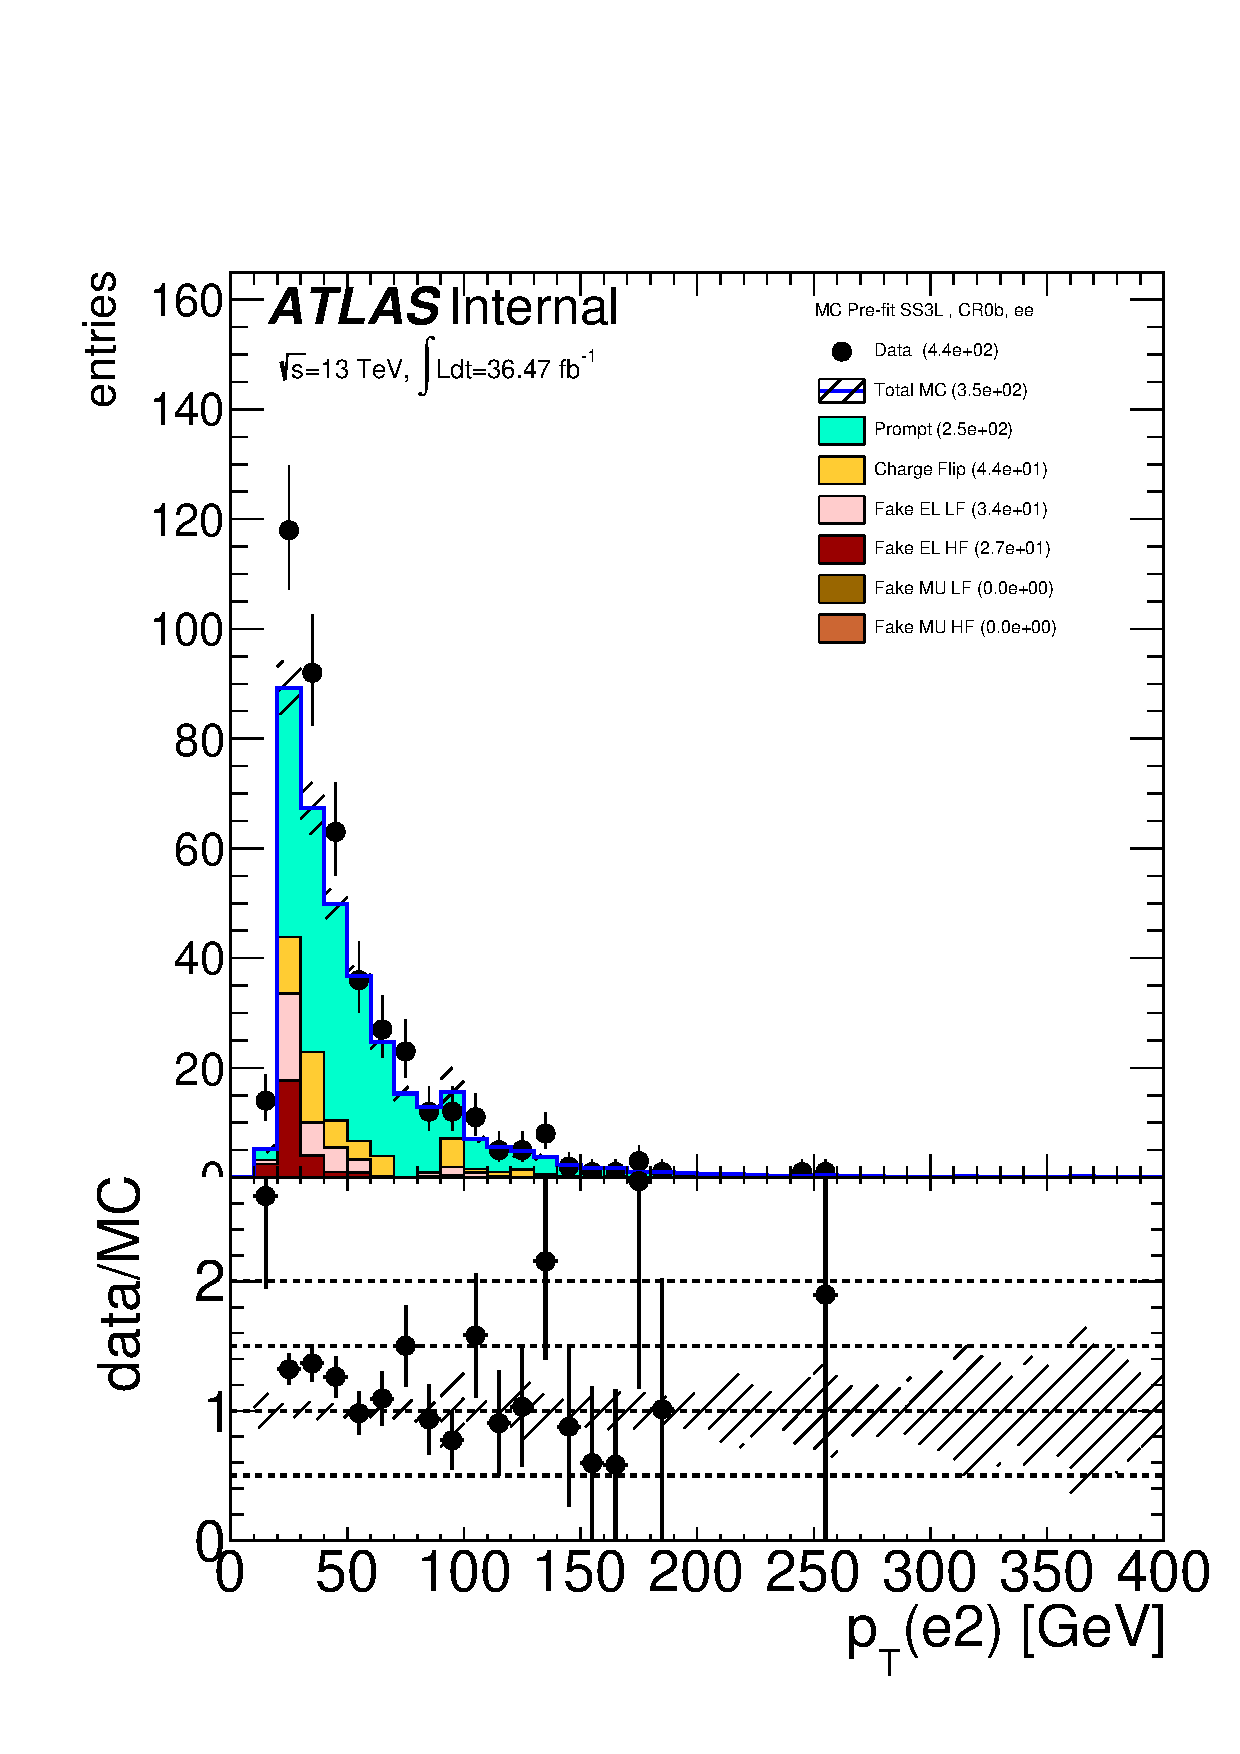
\includegraphics[width=.32\textwidth]{figures/mct/Prefit/el2_pt_ee_CR0b_SS3L}
   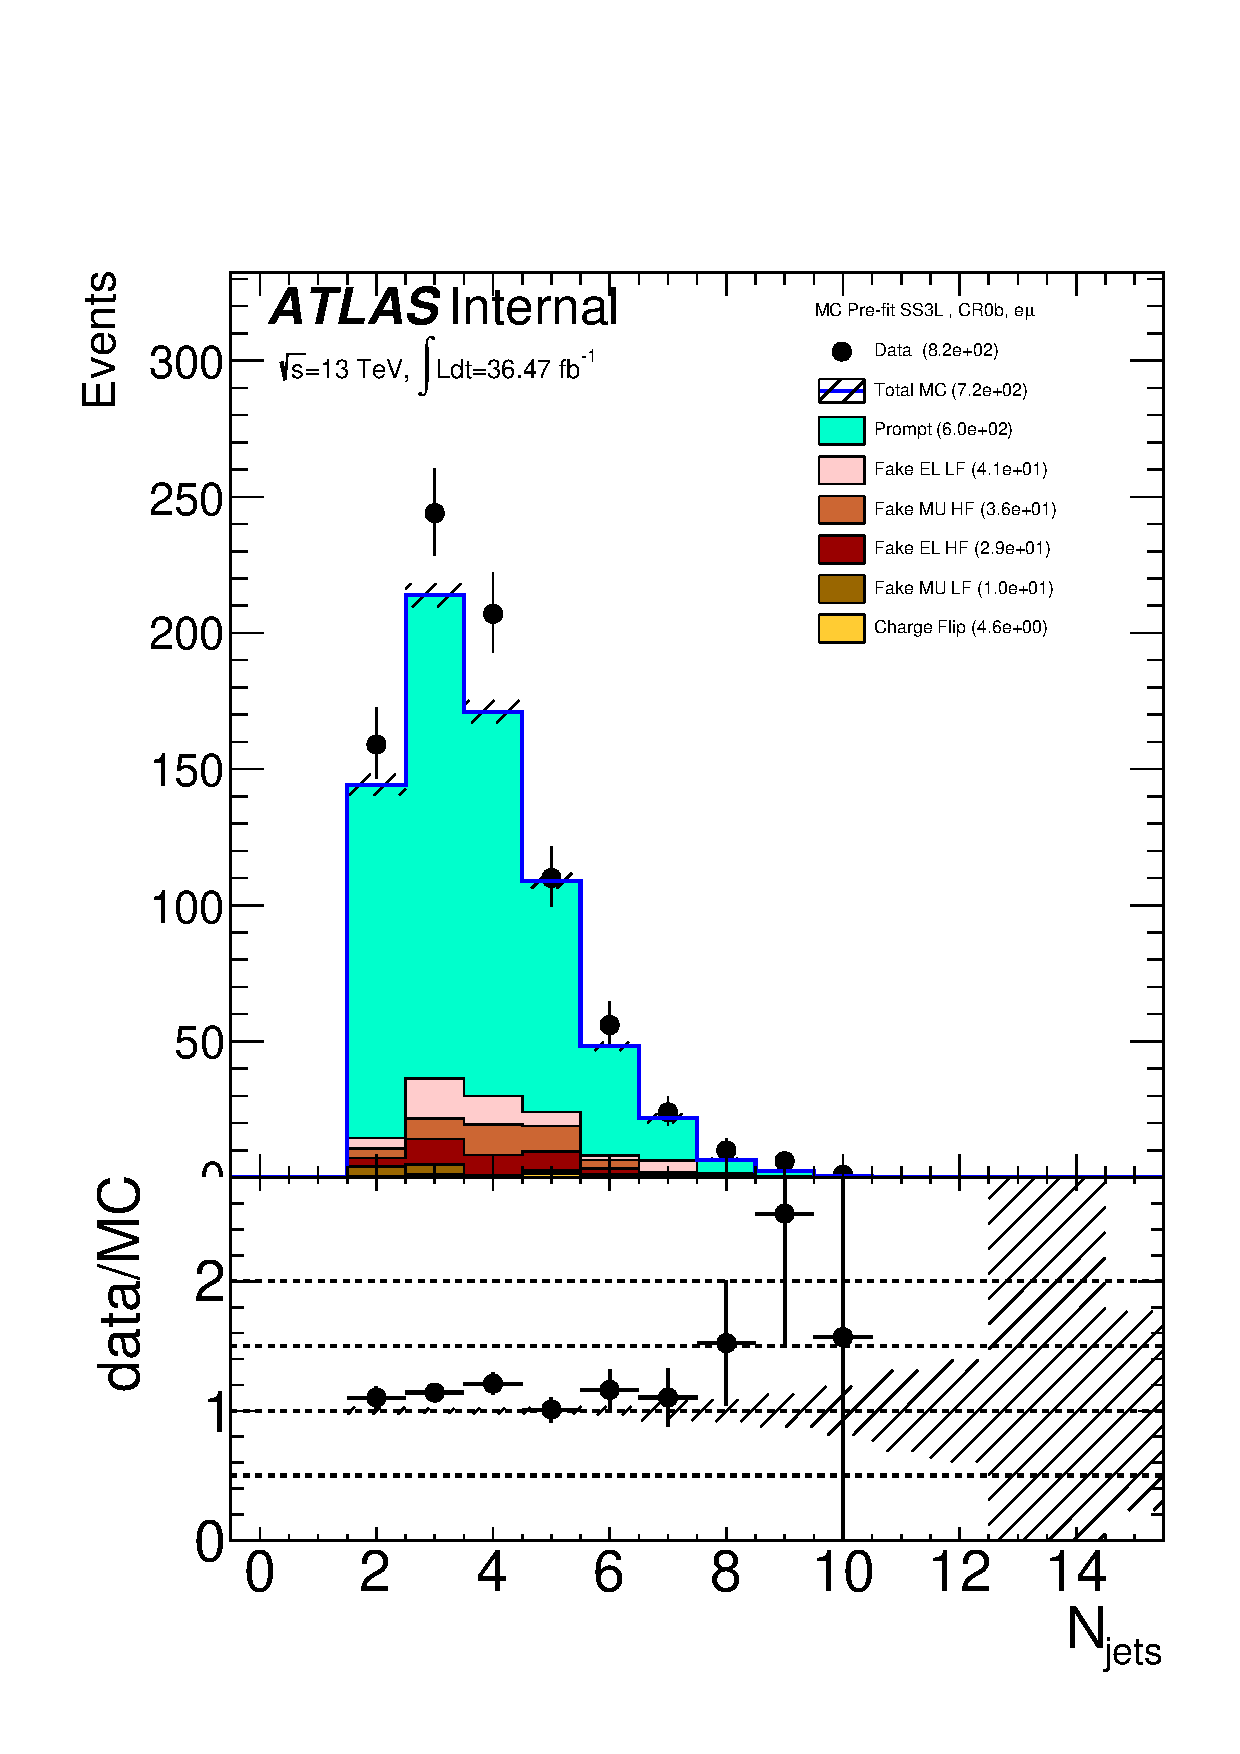
\includegraphics[width=.32\textwidth]{figures/mct/Prefit/NJETS_em_CR0b_SS3L}
   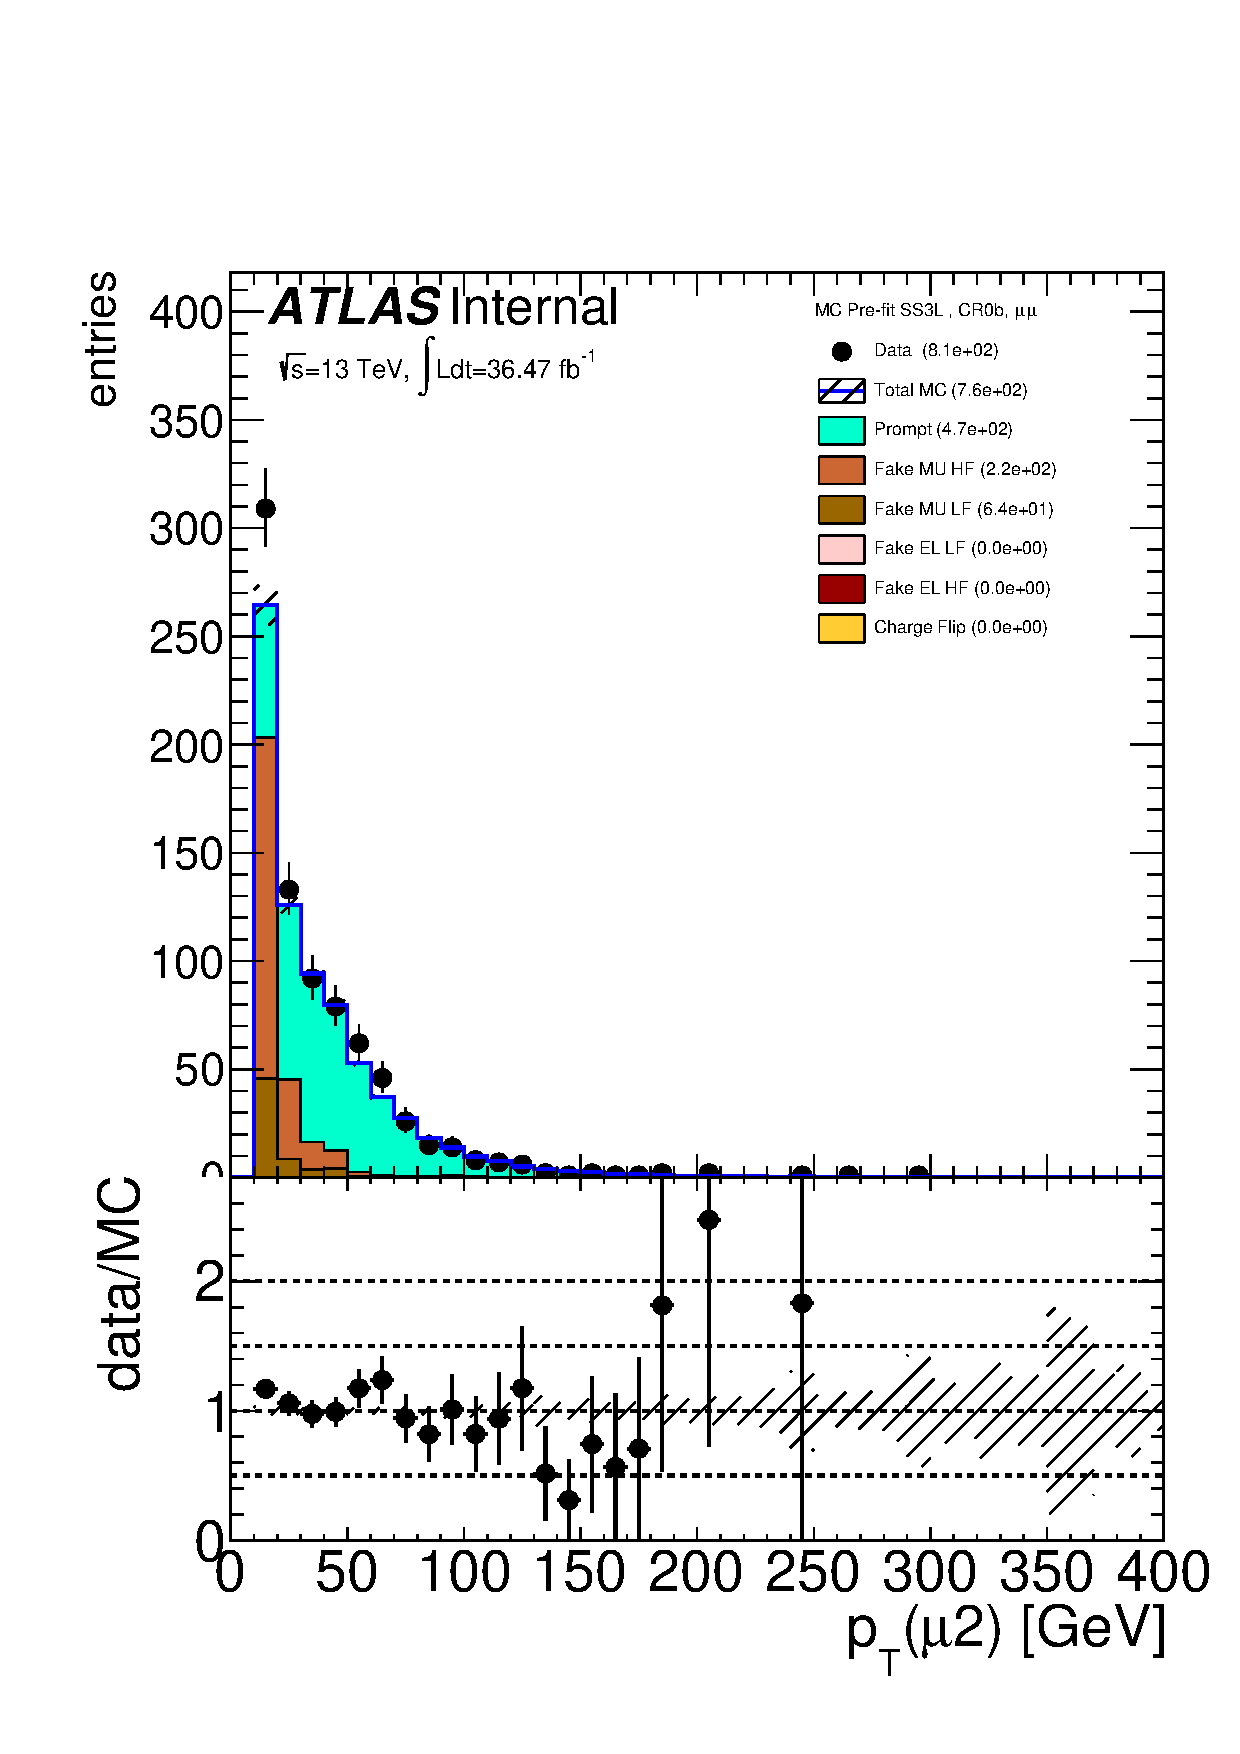
\includegraphics[width=.32\textwidth]{figures/mct/Prefit/mu2_pt_mm_CR0b_SS3L}
 \caption{
 Pre-fit distributions for  $ee$ channel (left),  for  $e\mu$ channel (middle), and  for  $\mu\mu$ channel (right) from CR0b that were used in the fit to extract the FNP lepton and charge flip multipliers.
The generator used in these plots is Powheg. The hashed band represents the sum of systematic uncertainties on the predictions.
 \label{f:prefit_CR0b}
 }
 \end{figure}

\begin{figure}[!htb]
  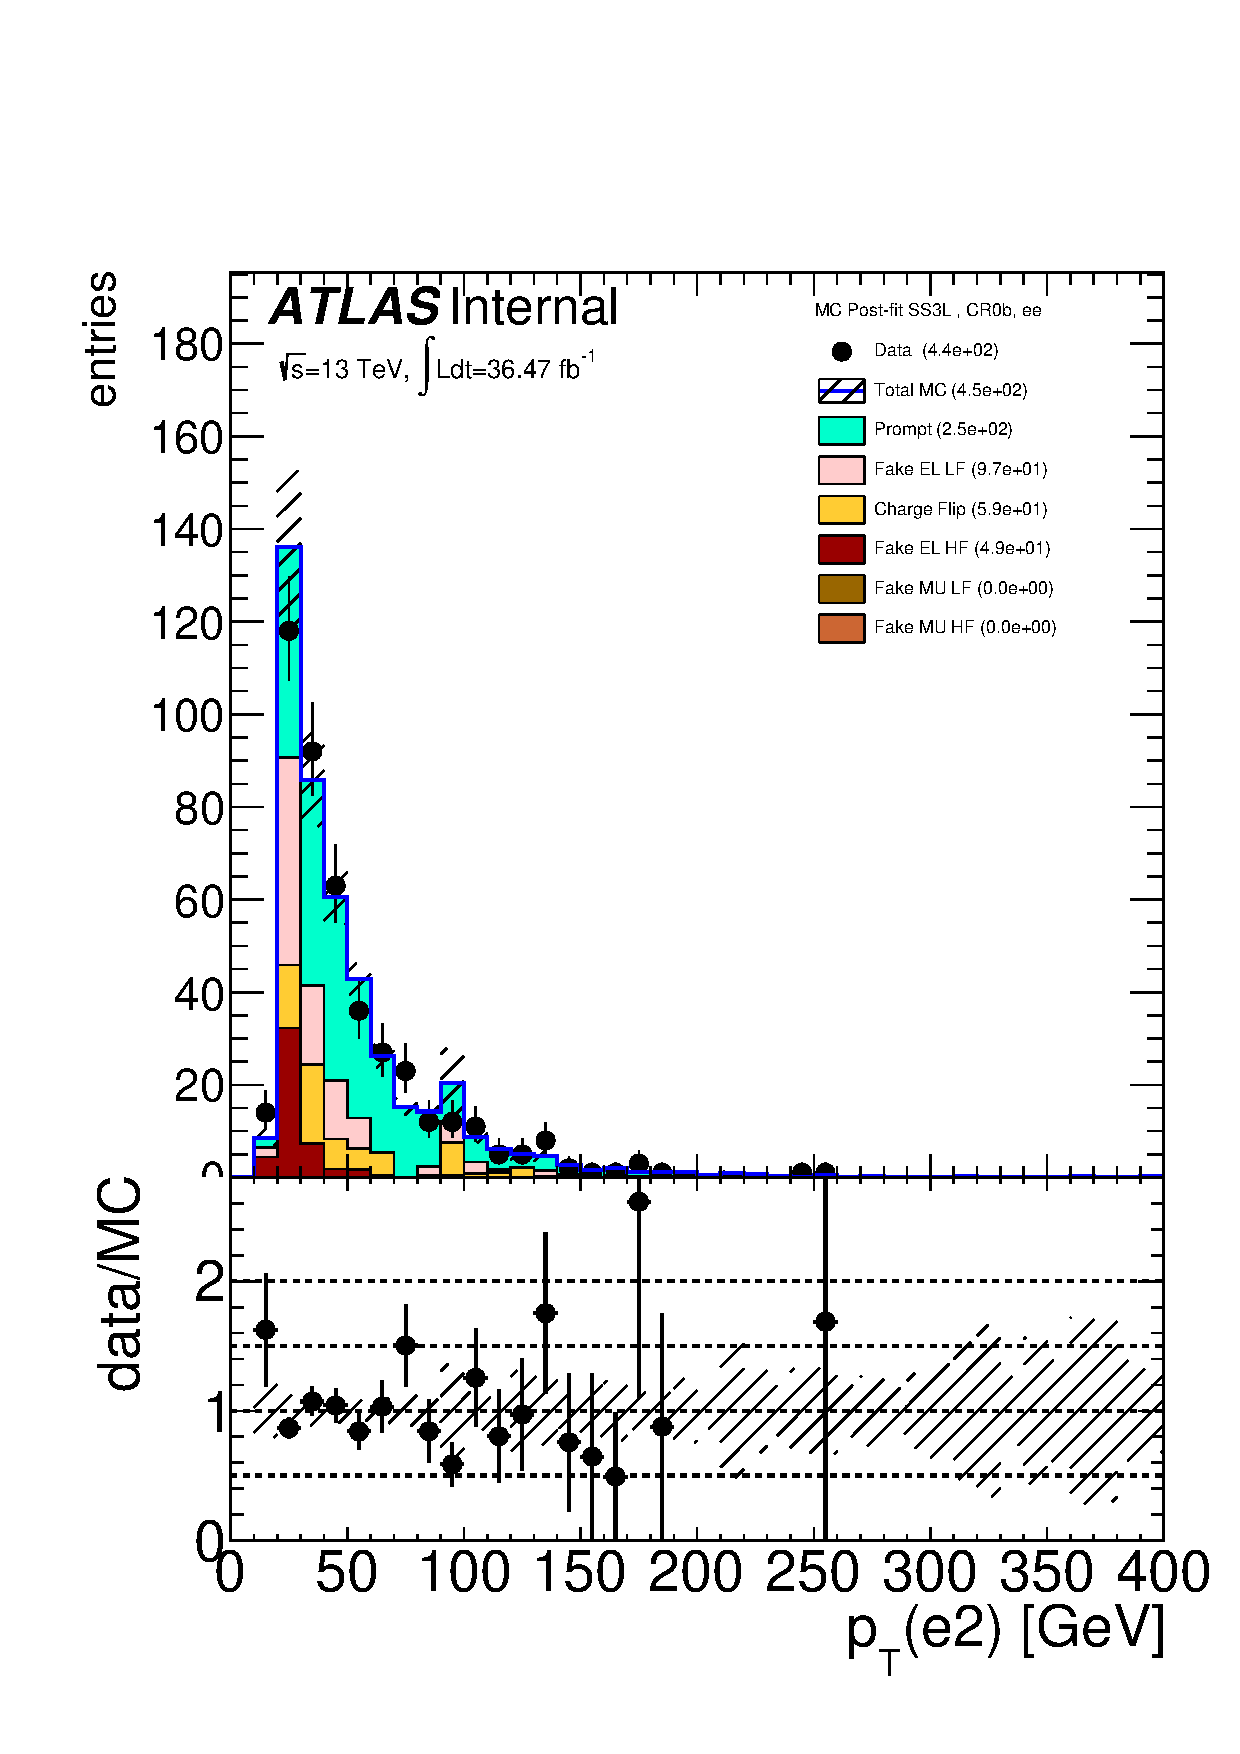
\includegraphics[width=.32\textwidth]{figures/mct/Postfit/el2_pt_ee_CR0b_SS3L}
  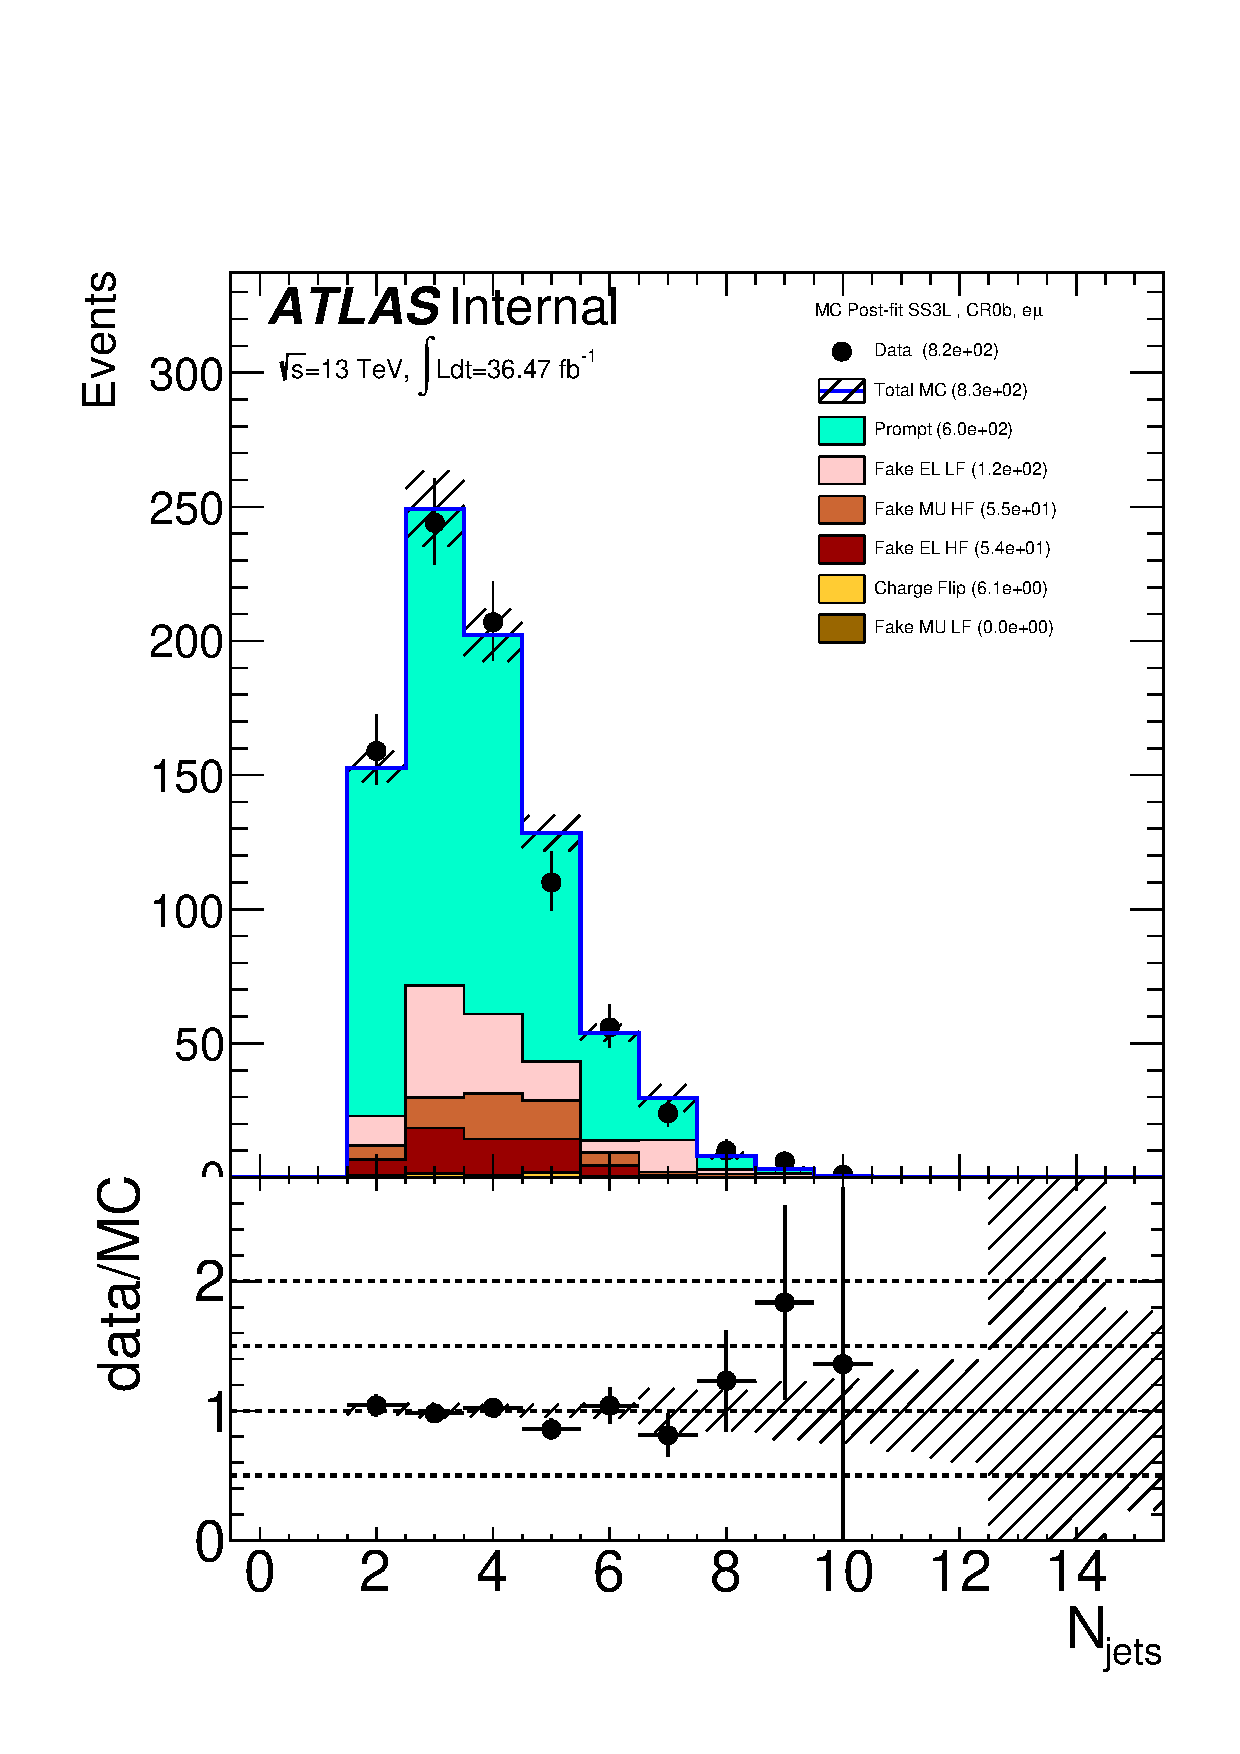
\includegraphics[width=.32\textwidth]{figures/mct/Postfit/NJETS_em_CR0b_SS3L}
  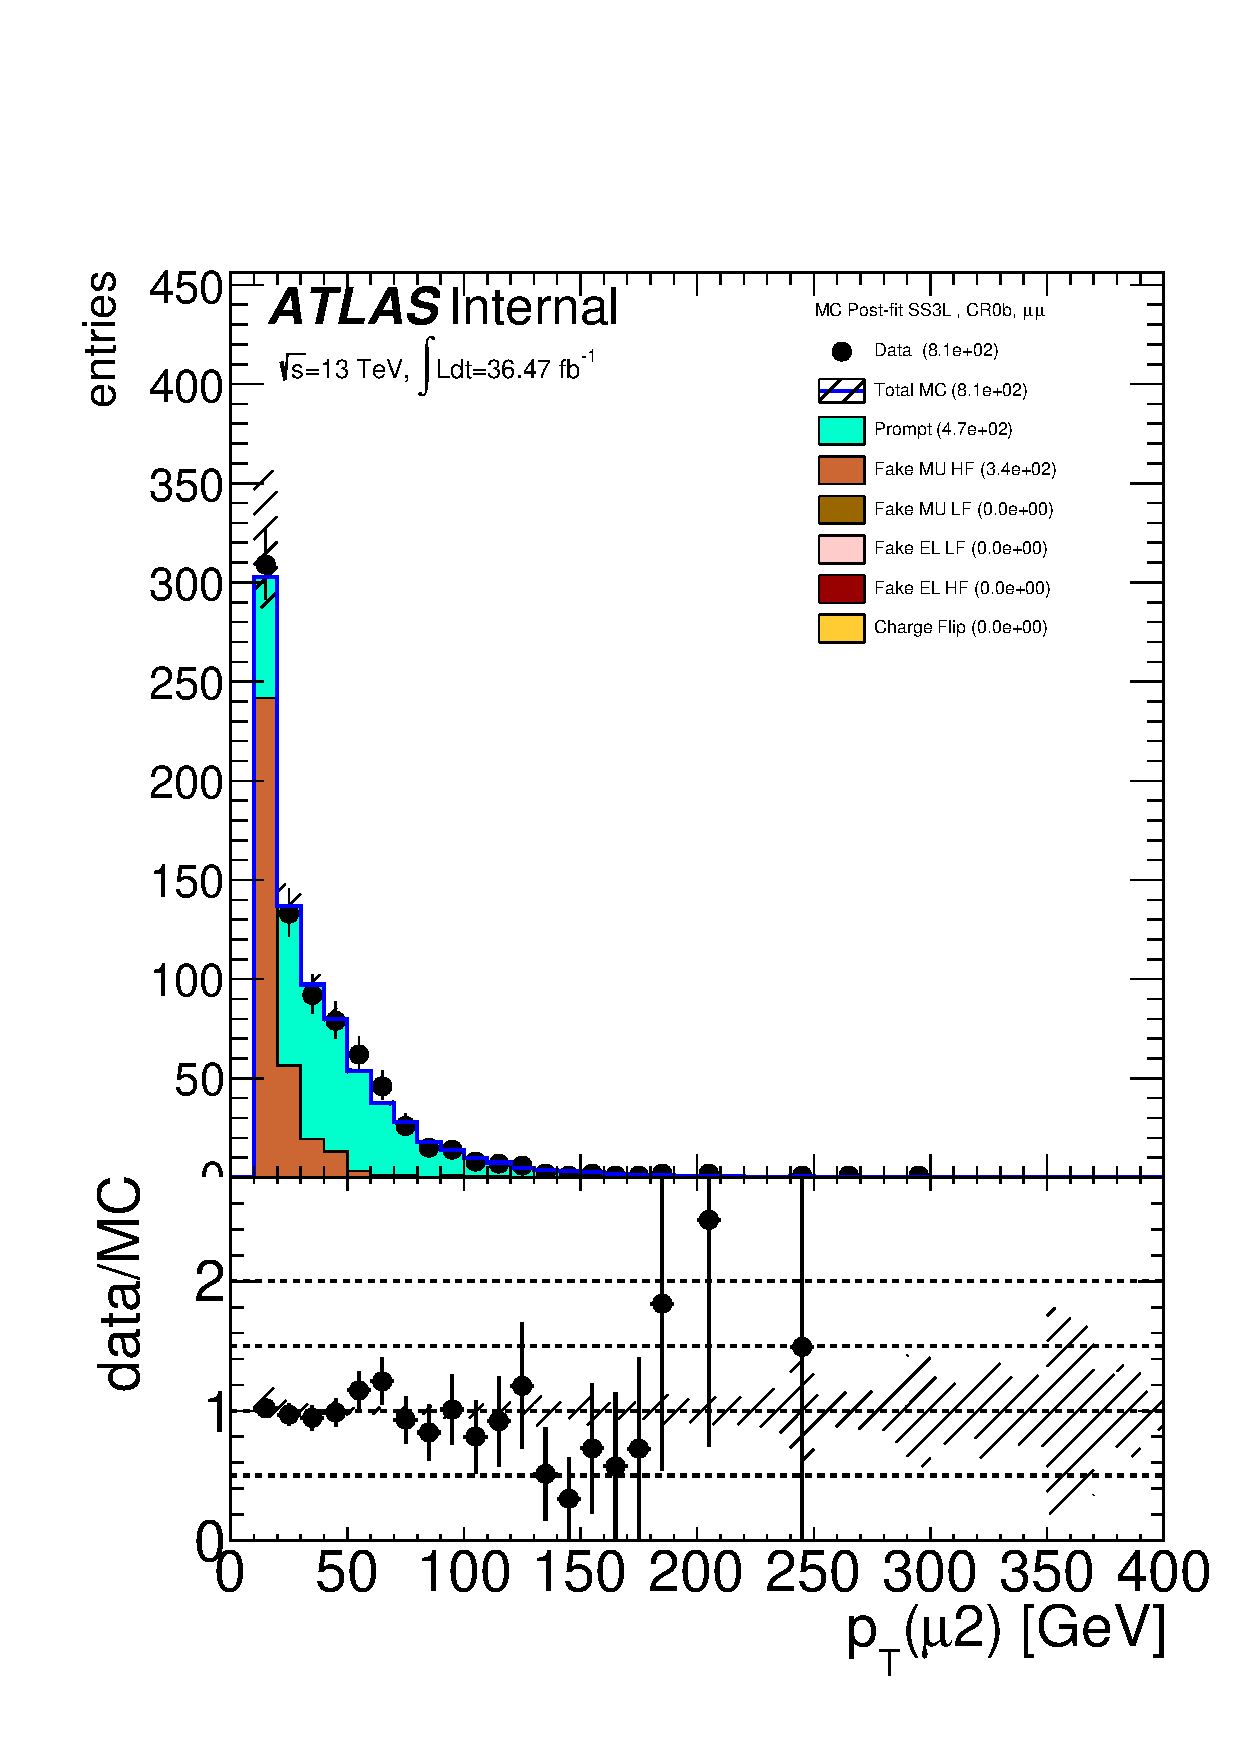
\includegraphics[width=.32\textwidth]{figures/mct/Postfit/mu2_pt_mm_CR0b_SS3L}
\caption{
Post-fit distributions for  $ee$ channel (left),  for  $e\mu$ channel (middle), and  for  $\mu\mu$ channel (right) from CR0b that were used in the fit to extract the FNP lepton and charge flip multipliers.
The generator used in these plots is Powheg. The hashed band represents the sum of systematic uncertainties on the predictions.
\label{f:postfit_CR0b}
}
\end{figure}

 \begin{figure}[!htb]
   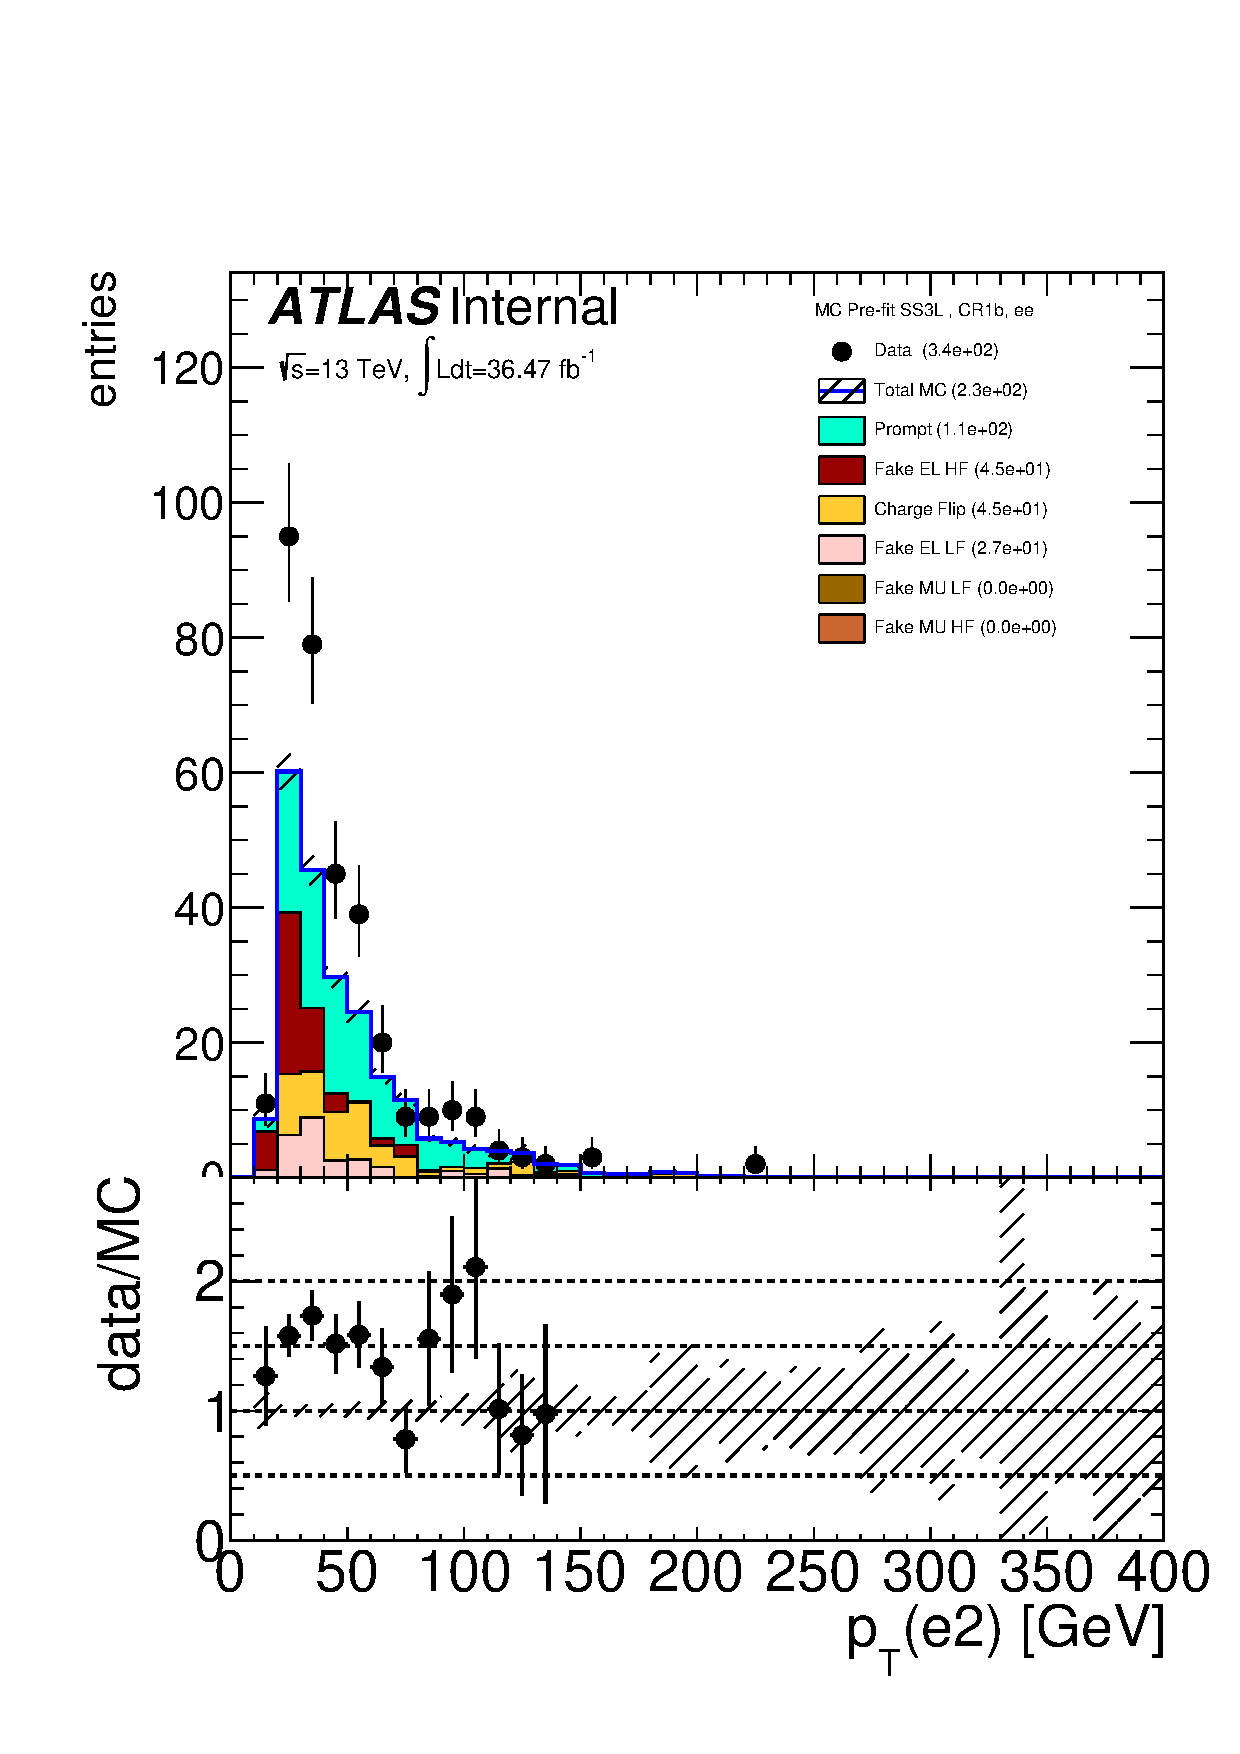
\includegraphics[width=.32\textwidth]{figures/mct/Prefit/el2_pt_ee_CR1b_SS3L}
   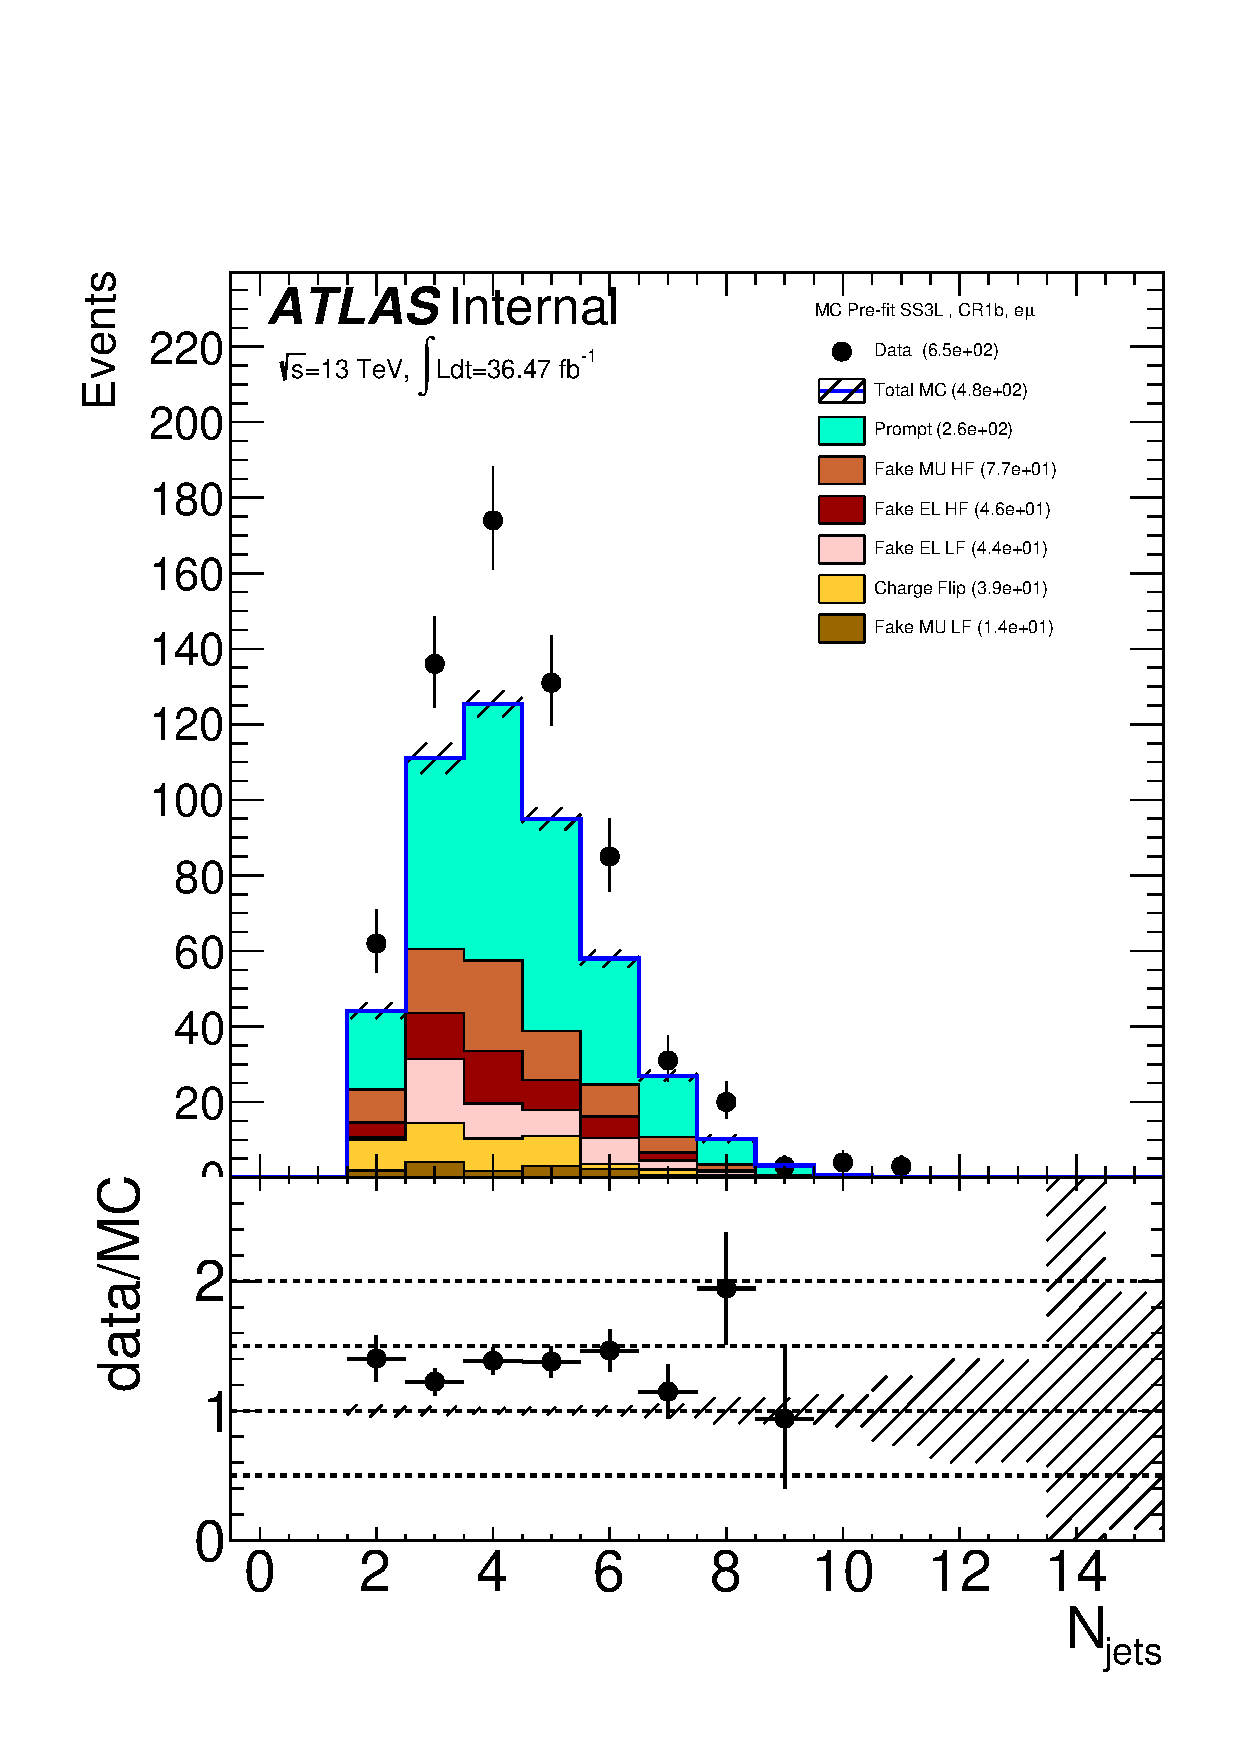
\includegraphics[width=.32\textwidth]{figures/mct/Prefit/NJETS_em_CR1b_SS3L}
   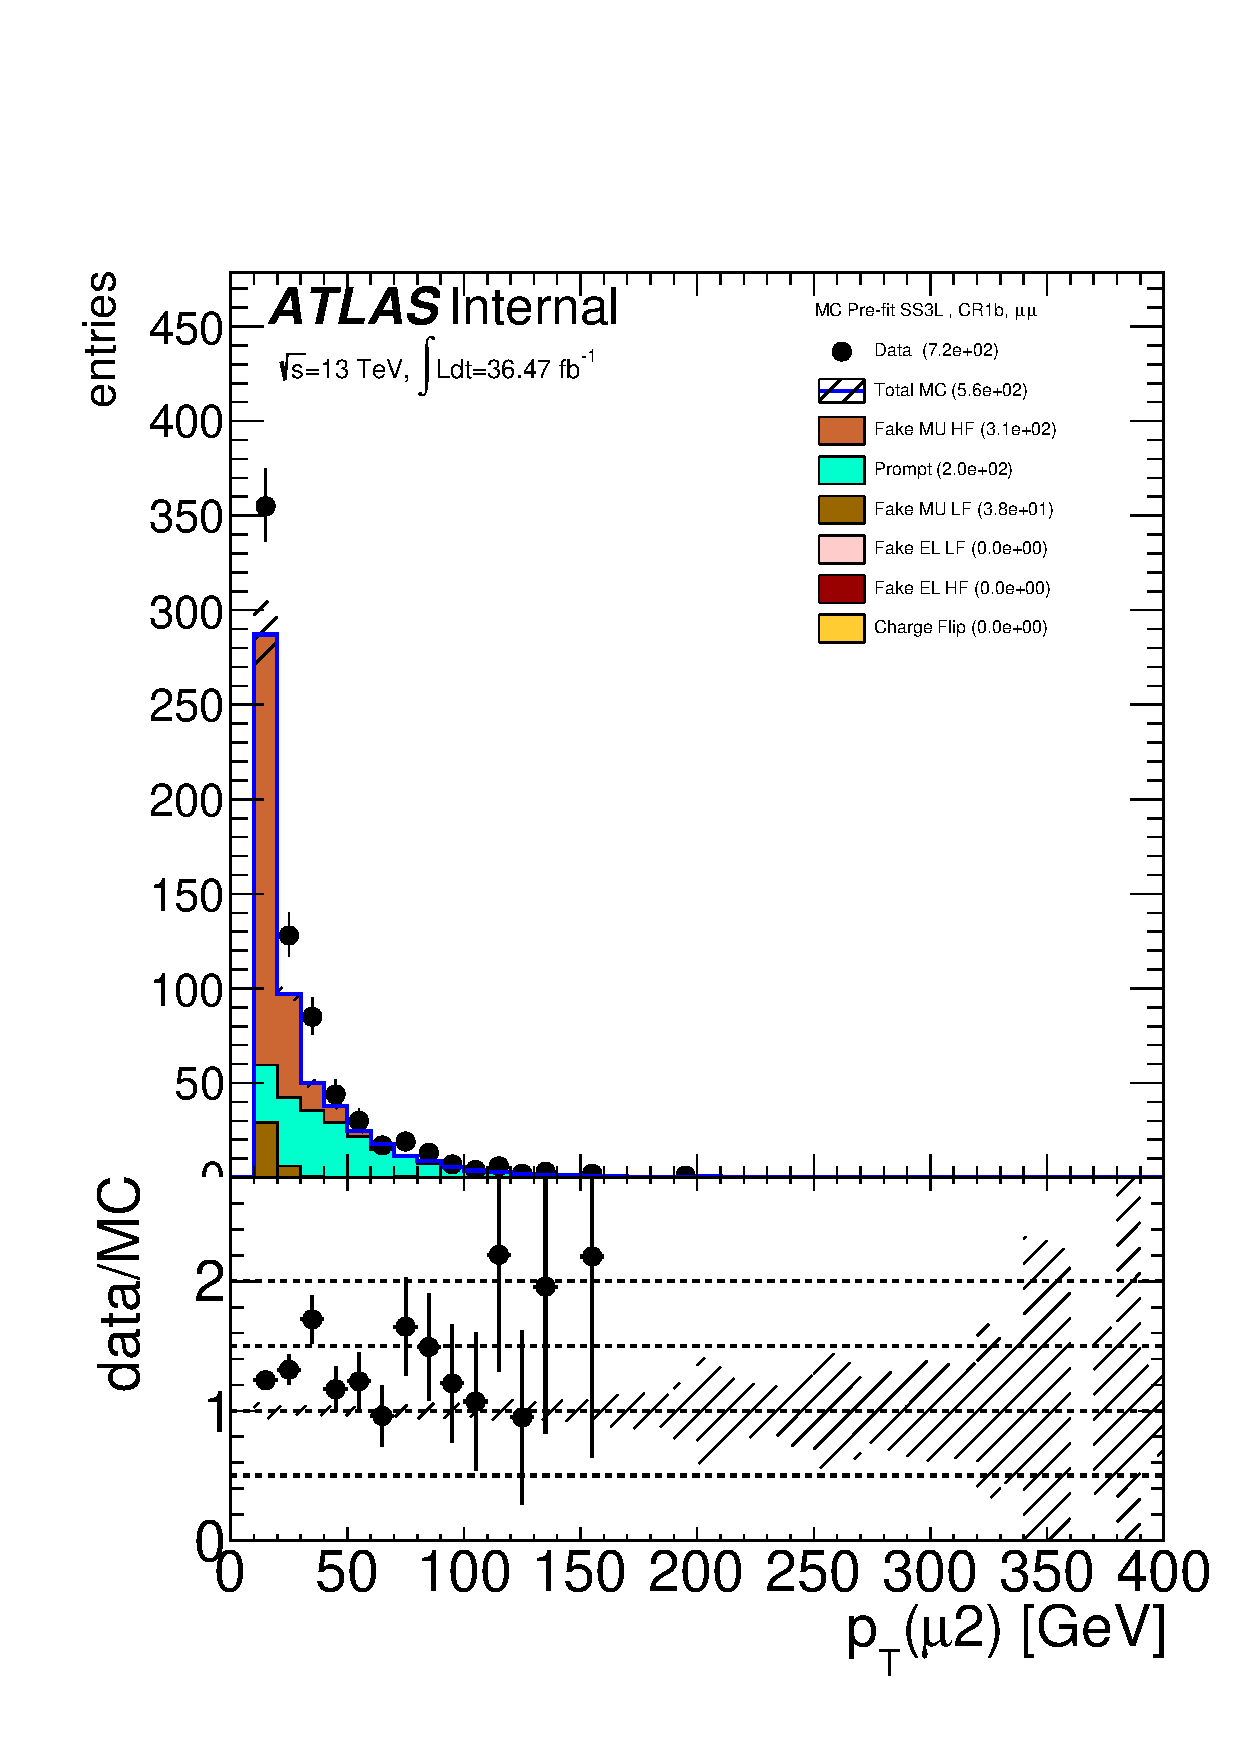
\includegraphics[width=.32\textwidth]{figures/mct/Prefit/mu2_pt_mm_CR1b_SS3L}
 \caption{
 Pre-fit distributions for  $ee$ channel (left), for  $e\mu$ channel (middle), and  for  $\mu\mu$ channel (right) from CR1b that were used in the fit to extract the FNP lepton and charge flip multipliers.
The generator used in these plots is Powheg. The hashed band represents the sum of systematic uncertainties on the predictions.
 \label{f:prefit_CR1b}
 }
 \end{figure}

\begin{figure}[!htb]
  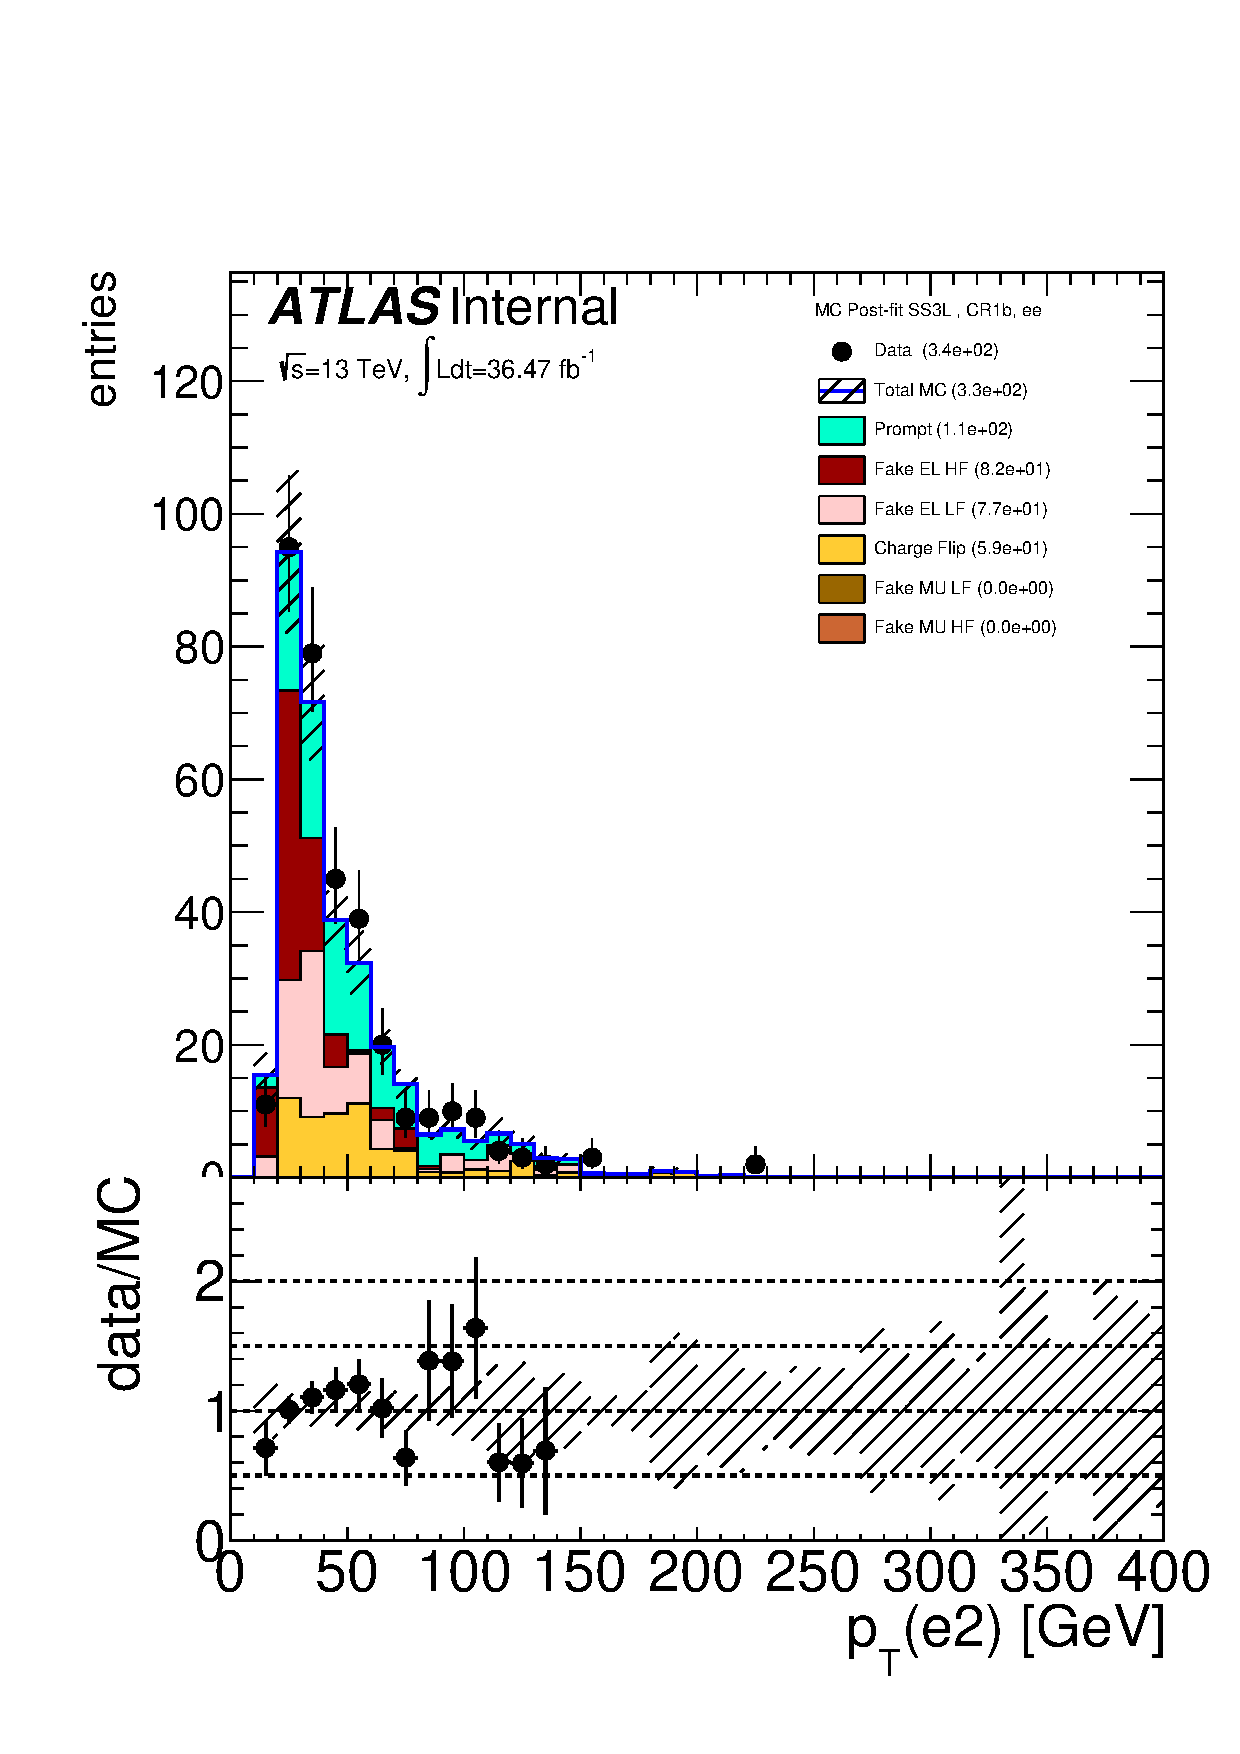
\includegraphics[width=.32\textwidth]{figures/mct/Postfit/el2_pt_ee_CR1b_SS3L}
  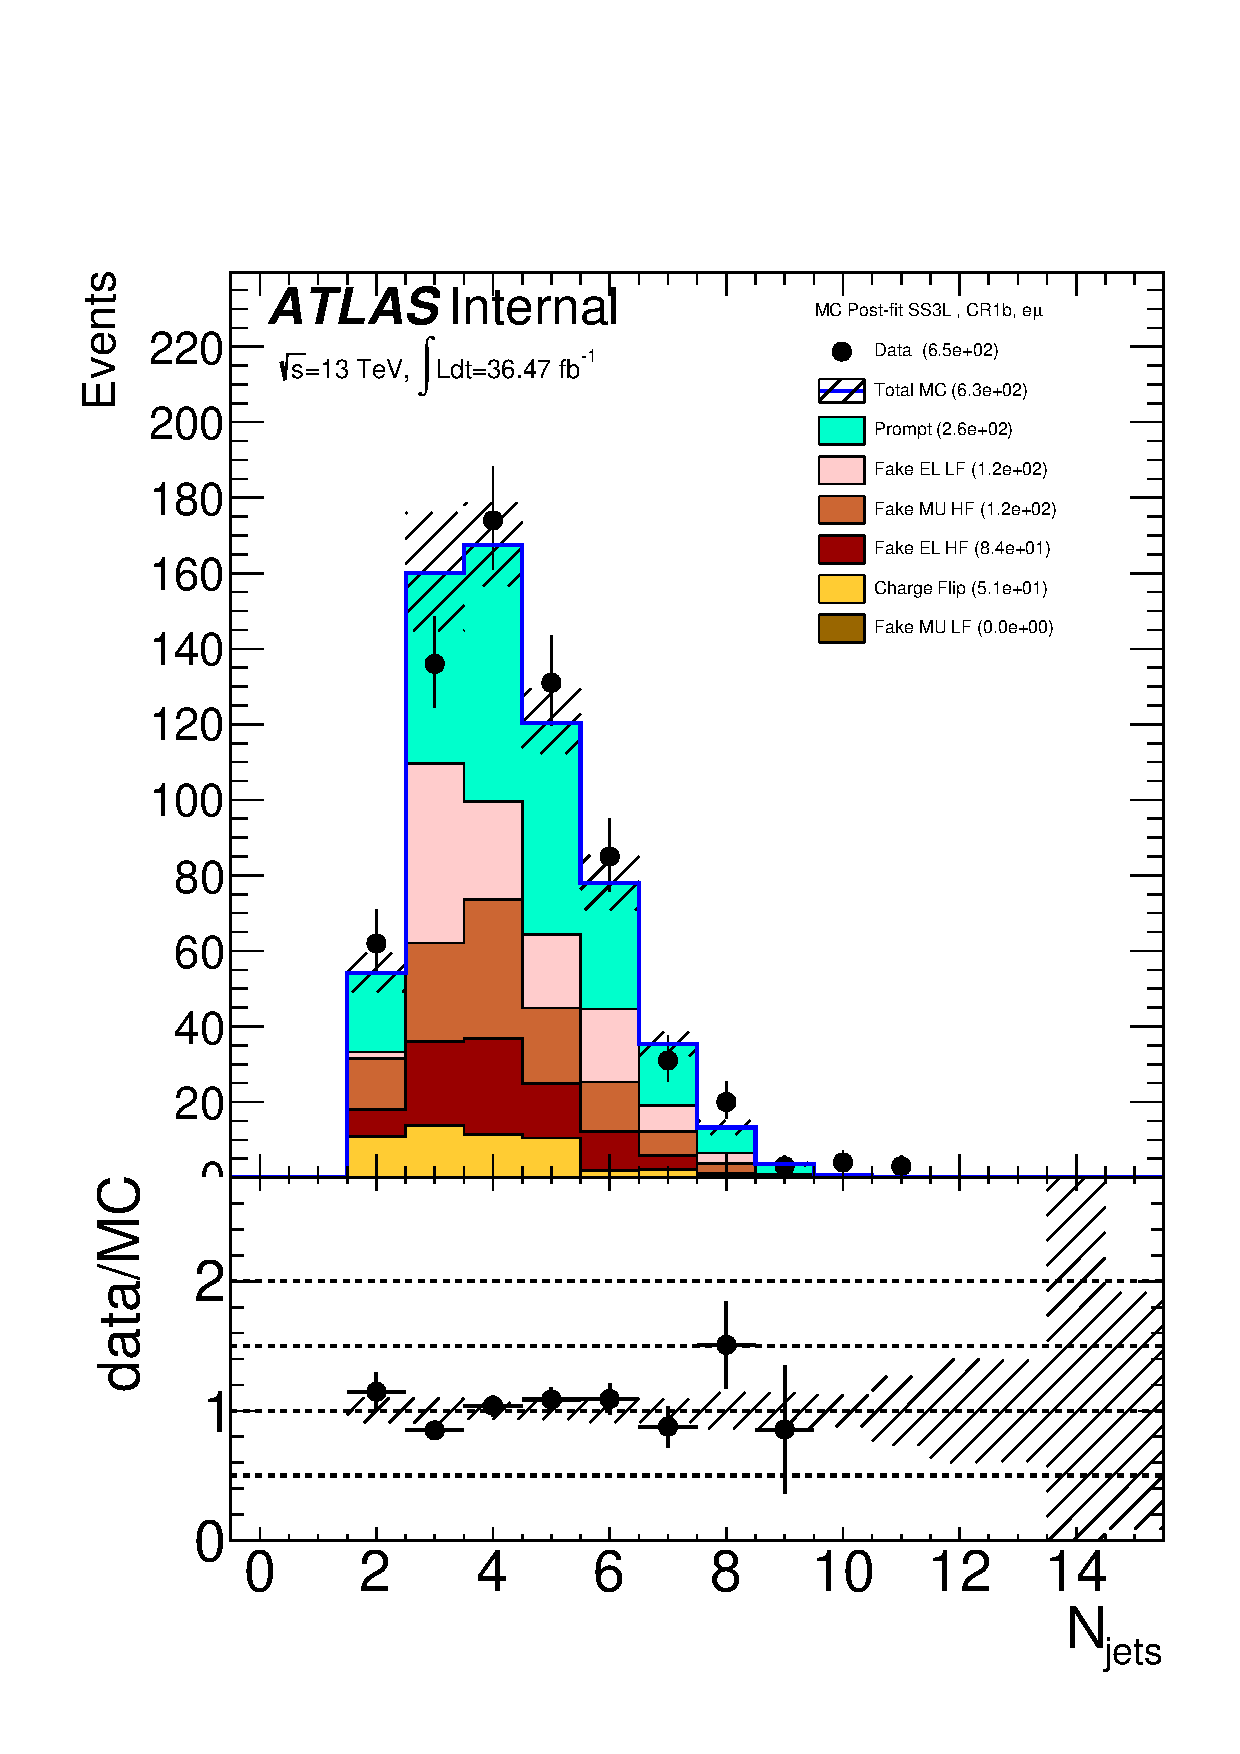
\includegraphics[width=.32\textwidth]{figures/mct/Postfit/NJETS_em_CR1b_SS3L}
  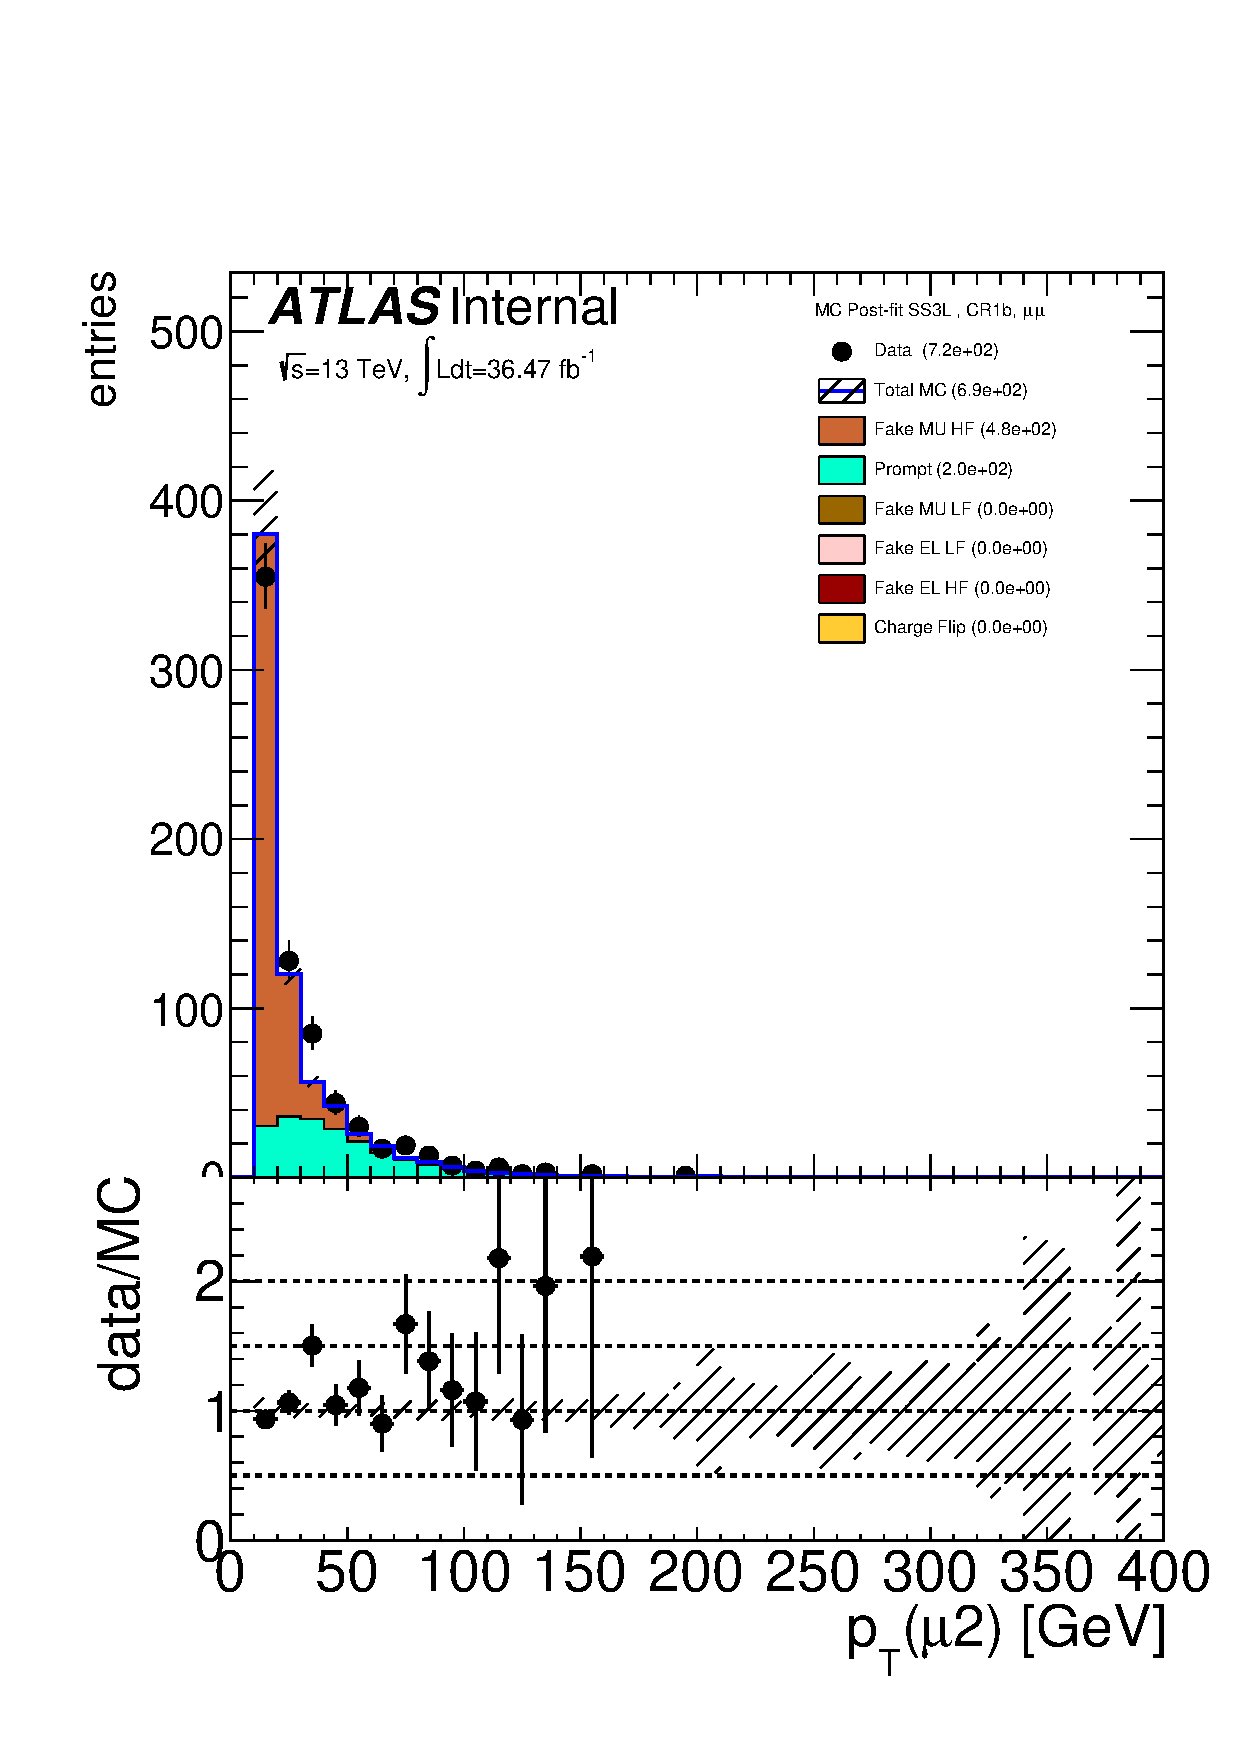
\includegraphics[width=.32\textwidth]{figures/mct/Postfit/mu2_pt_mm_CR1b_SS3L}
\caption{
Post-fit distributions for  $ee$ channel (left), for  $e\mu$ channel (middle), and  for  $\mu\mu$ channel (right) from CR1b that were used in the fit to extract the FNP lepton and charge flip multipliers.
The generator used in these plots is Powheg. The hashed band represents the sum of systematic uncertainties on the predictions.
\label{f:postfit_CR1b}
}
\end{figure}

The minimization of the negative log likelihood using the \textsc{Minuit} package leads 
to the multipliers shown in Tables \ref{t:fake_factors_powheg} and \ref{t:fake_factors_sherpa}.
The tables represent the multipliers obtained from the fit upon using two different parton showers, \POWHEGBOX and \SHERPA 
for the processes that lead to FNP leptons and charge flips.
The systematic uncertainty is obtained by varying the 
generator from \POWHEGBOX to \SHERPA and evaluating the impact on the expected background from FNP and charge flip leptons. 
It is found to be the dominant contribution to the systematic uncertainty of the method (up to 80\%).
The uncertainties in the multipliers themselves correspond to how much the parameter needs to be varied for 
a one standard deviation change in the likelihood function. This uncertainty takes into account the limited number of simulated events and is included as a 
systematic uncertainty on the expected number of background events. 

\begin{table}[!htb]
  \caption{The FNP and charge flip multipliers obtained after minimizing the likelihood function using Pythia.
    The uncertainty in the multipliers takes into account the limited statistics of simulated events.
    \label{t:fake_factors_powheg}}
  \centering
  % % \scalebox{0.85}{
   \begin{tabular}{|c|c|c|}
          \hline
          Category & Multiplier & Uncertainty  \\
          \hline
          chFlip & 1.49 & 0.58 \\ 
          HF EL & 2.80 & 0.98 \\
          LF EL & 2.89 & 0.88 \\
          HF MU & 1.59 & 0.31 \\
          LF MU & 1.00 & 1.34 \\
          \hline
        \end{tabular}
  % % }                                                                            
\end{table}

\begin{table}[!htb]
  \caption{The FNP and charge flip multipliers obtained after minimizing the likelihood function using Sherpa.
    The uncertainty in the multipliers takes into account the limited statistics of simulated events.
    \label{t:fake_factors_sherpa}}
  \centering
  % % \scalebox{0.85}{
  \begin{tabular}{|c|c|c|}
    \hline
    Category & Multiplier & Uncertainty  \\
    \hline
    chFlip & 1.34 & 0.58 \\ 
    HF EL & 2.40 & 0.85 \\
    LF EL & 1.83 & 1.04 \\
    HF MU & 1.17 & 0.16 \\
    LF MU & 2.40 & 0.81 \\
    \hline
  \end{tabular}                                                                                         
  % % }                                                                            
\end{table}



\section{Matrix Method}


The FNP leptons do not often pass one of the 
lepton selection criteria but have non-zero impact parameter, and are often not 
well-isolated. These selection requirements are key ingredients to control the FNP leptons. 
The number of events with at least one FNP lepton is estimated using two classes of leptons: 
a real-enriched class of ``tight'' leptons corresponding to signal leptons and a fake-enriched class of ``loose'' leptons 
corresponding to candidate leptons with relaxed identification criteria\footnote{Signal leptons are leptons satisfying the signal lepton definition, while the candidate leptons are leptons satisfying some pre-selection cuts and usually passing the overlap removal requirements as discssed in the analysis section ??.}. 
In the next sections, a description of the simplest form of the matrix method will be given with events containing one object. 
Then a generalized treatment that can handle events with an arbitrary number of leptons in the final states will be discussed.

\subsection{Events with one object}

Given the probabilities $\varepsilon/\zeta$ for a real/FNP candidate lepton to satisfy the signal lepton criteria, 
one can relate the number of events with one candidate lepton passing/failing signal requirements ($n_\text{pass}/n_\text{fail}$) to the number of events with one real/FNP signal leptons ($n_\text{real}/n_\text{FNP}$):

\begin{align}
\begin{pmatrix}n_\text{pass}\\n_\text{fail}\end{pmatrix} 
= \begin{pmatrix}\varepsilon & \zeta\\ 1-\varepsilon & 1-\zeta\end{pmatrix}
\begin{pmatrix}n_\text{real}\\n_\text{FNP}\end{pmatrix}; 
\label{eqn:matrix_method}
\end{align}
allowing to determine the unknown number of events $n_\text{FNP}$ from the observed $n_\text{pass}$ and $n_\text{fail}$ given measurements of the 
probabilities $\varepsilon/\zeta$. 

The predictive power of the matrix method comes from the fact that 
the real and FNP leptons have different composition in the two collections 
of tight and loose objets leading to $\varepsilon \neq \zeta$. In fact, 
the tight lepton collection will be dominated by real objects while the 
loose region will be dominated by fake objects. As a result, 
the inequality $\varepsilon >> \zeta$ will always hold true which 
guarantees that the martrix in Eq. \ref{eqn:matrix_method} is invertible 
and gives positive estimates. 

The next step is to invert the relation in Eq. \ref{eqn:matrix_method} to 
obtain

\begin{align}
\begin{pmatrix}n_\text{real}\\n_\text{FNP}\end{pmatrix} 
= \frac{1}{\varepsilon - \zeta} \begin{pmatrix}\bar\zeta & -\zeta\\ -\bar\varepsilon & \varepsilon\end{pmatrix}
\begin{pmatrix}n_\text{pass}\\n_\text{fail}\end{pmatrix}; 
\label{eqn:fake.inv_matrix_method}
\end{align}

where $\bar\varepsilon = 1 - \varepsilon$ and  $\bar\zeta = 1 - \zeta$. 
The FNP lepton component is: 

\begin{align}
n_\text{FNP} = \frac{1}{\varepsilon - \zeta}\left(\left(\varepsilon-1\right)n_\text{pass}+n_\text{fail}\right).
\label{eqn:fake.nfake}
\end{align}

However, the quantity of interest is the expected FNP lepton background that 
passes the tight selection criteria: 
$n_{\text{pass}~\cap~\text{FNP}} = \zeta n_\text{FNP}$.
 To obtain this quantity, 
the identity from Eq. \ref{eqn:matrix_method} is used to get:

\begin{align}
n_\text{FNP} = \frac{\zeta}{\varepsilon - \zeta}\left(\left(\varepsilon-1\right)n_\text{pass}+n_\text{fail}\right).
\label{eqn:fake.nFNPpass}
\end{align}

The linearity of Eq. \ref{eqn:fake.nFNPpass}  with respect to $n_\text{pass}$ 
and $n_\text{fail}$ allows the method to be applied on an event-by-event, 
effectively resulting into a weight being assigned to each event. 
By defining
\[
  n_\text{pass} = \sum_\text{all events} \mathbb{1}_\text{pass},~
  n_\text{fail} = \sum_\text{all events} \mathbb{1}_\text{fail},~ 
  \mathbb{1}_\text{fail} = 1 -  \mathbb{1}_\text{pass},
\]
where $\mathbb{1}_{\text{pass} \left(\text{fail}\right)} = 1$ if the object pass (fail) the tight selection requirement and $\mathbb{1}_{\text{pass}\left(\text{fail}\right)} = 0$ otherwise. Eq. \ref{eqn:fake.nFNPpass} can be written as


\[
n_\text{FNP} = \sum_\text{all events} \{
\frac{\zeta}{\varepsilon - \zeta}\left(\varepsilon - 
\mathbb{1}_\text{pass}\right)
\}
\\
=  \sum_\text{all events} \omega
\]

where 

\begin{align}
  \omega = \frac{\zeta}{\varepsilon - \zeta}\left(\varepsilon - 
\mathbb{1}_\text{pass}\right)
  \label{eqn:fake.nFNPpass.demo}
\end{align}

is the weight to be assigned to each event in the case of one FNP lepton 
in the event. 
The generalization of this formalism to higher dimensions 
with multiple objects will be covered next.



\subsection{Dynamic matrix method}


The one lepton case readily generalizes to events with more than one lepton
in a formalism that can handle an arbitrary number of leptons 
in the event. The method should be applied event-by-event, effectively 
resulting into a weight being assigned to each event. The predicted yield of 
events with FNP leptons is simply the sum of weights.
A general formula will be derived starting from the two objects case 
then specific examples will be given to illustrate the application of the 
method.

If two objects are present in the event, the probabilites $\varepsilon/\zeta$
will depend on the kinematic properties of these objects. Typically 
the probabilies will vary as a function of \pt and $|\eta|$. For this reason,
the probabilities will be different and will have an index to 
identify the object under study: 
 $\varepsilon_i/\zeta_i$ where $i=1,2...$. 
%% For example, events with 
%% two leptons where the probabilities are measured in 3 bins of \pt and 
%% 2 bins of $\eta$ can be placed in one of twelve categories. 
An identity similar to Eq.  \ref{eqn:matrix_method} can be formed for 
two objects with a change in notation for simplicity:

\begin{align}
\left(\begin{array}{c}
N_{TT} \\  N_{TL} \\ N_{LT} \\ N_{LL}
\end{array}\right) = 
\Lambda \times 
\left(\begin{array}{c}
N_{RR} \\  N_{RF} \\ N_{FR} \\ N_{FF}
\end{array}\right), 
\label{eq:mxm_start}
\end{align}
where $(N_{RR},N_{RF},N_{FR},N_{FF})$ are the number of events with respectively two real, one real plus one FNP (two terms), and two FNP leptons before applying tight cuts, respectively, and $(N_{TT},N_{TL},N_{LT},N_{LL})$ are the observed number of events for which respectively both lepton pass the tight cut, only one of them (two terms), or both fail the tight cut, respectively. 

$\Lambda$ is given by:
\[
\Lambda=
\left(\begin{array}{cccc}
\varepsilon_1\varepsilon_2 & \varepsilon_1\zeta_2 & \zeta_1\varepsilon_2 & \zeta_1\zeta_2\\
\varepsilon_1(1-\varepsilon_2) & \varepsilon_1(1-\zeta_2) & \zeta_1(1-\varepsilon_2) & \zeta_1(1-\zeta_2)\\
(1-\varepsilon_1)\varepsilon_2 & (1-\varepsilon_1)\zeta_2 & (1-\zeta_1)\varepsilon_2 & (1-\zeta_1)\zeta_2\\
(1-\varepsilon_1)(1-\varepsilon_2) & (1-\varepsilon_1)(1-\zeta_2) & (1-\zeta_1)(1-\varepsilon_2) & (1-\zeta_1)(1-\zeta_2)
\end{array}\right) 
\]
which can also be written in terms of a Kronecker product in 
Eq. \ref{eq:mxm_start} to obtain:
\begin{align}
\left(\begin{array}{c}
N_{TT} \\  N_{TL} \\ N_{LT} \\ N_{LL}
\end{array}\right)
= \begin{pmatrix}\varepsilon_1 & \zeta_1\\ \bar\varepsilon_1 & \bar\zeta_1\end{pmatrix} \bigotimes \begin{pmatrix}\varepsilon_2 & \zeta_2\\ \bar\varepsilon_2 & \bar\zeta_2\end{pmatrix}
\left(\begin{array}{c}
N_{RR} \\  N_{RF} \\ N_{FR} \\ N_{FF}
\end{array}\right)
\label{eq:mxm_start_kroe}
\end{align}
To make the notation more compact, the set of 4 numbers $(N_{TT},N_{TL},N_{LT},N_{LL})$ can be represented by a rank 2 tensor $\mathcal{T}_{\alpha_1 \alpha_2}$ 
where $\alpha_i$ corresponds to one object that is either tight (T) or 
loose (L). 
Similarly the numbers $(N_{RR},N_{RF},N_{FR},N_{FF})$ can be represented 
by $\mathcal{R}_{\alpha_1 \alpha_2}$ where $\alpha_i$ corresponds to one object 
that is either real (R) or FNP (F). With this convention, the 
Kronecker product of Eq. \ref{eq:mxm_start_kroe} can be obtained by 
contracting each index $\alpha_i$ of the tensors $\mathcal{T}$ or $\mathcal{R}$
by the 2 $\times$ 2 matrix $\phi_i\tensor{\vphantom{\phi}}{_{\beta_i}^{\alpha_i}}$:


\begin{align}
\mathcal{T}_{\beta_1 \beta_2} = 
\phi_1\tensor{\vphantom{\phi}}{_{\beta_1}^{\alpha_1}} 
\phi_2\tensor{\vphantom{\phi}}{_{\beta_2}^{\alpha_2}}
\mathcal{R}_{\alpha_1 \alpha_2},~
\phi_i = 
 \begin{pmatrix}\varepsilon_i & \zeta_i\\ \bar\varepsilon_i & \bar\zeta_i\end{pmatrix}
\label{eq:fake.tensor_compact}
\end{align}

Following the same procedure as in the one object case, the matrix inversion 
of the 4$\times$4 $\lambda$ matrix is simplified to a matrix inversion of 
the 2$\times$2 $\phi$ matrices. The quantity of interest is the FNP lepton 
background that passes the tight selection criteria as in 
Eq. \ref{eqn:fake.nFNPpass} which can be compactly written in the 
two objects case as: 

\begin{align}
\mathcal{T}_{\nu_1 \nu_2}^\text{FNP} = 
\phi\indices{_{\nu_1}^{\mu_1}} 
\phi\indices{_{\nu_2}^{\mu_2}}
\tensor*{\xi}{*^{\beta_1}_{\mu_1}^{\beta_2}_{\mu_2}}
\phi\indices{^{-1}_{\beta_1}^{\alpha_1}} 
\phi\indices{^{-1}_{\beta_2}^{\alpha_2}}
\mathcal{T}_{\alpha_1 \alpha_2}.
\label{eq:fake.FNP_compact}
\end{align}

The tensor $\xi$ encodes the component of tight and FNP lepton background. 
In the two objects case, $\xi$ needs to select the total background 
with at least one fake lepton $N_F = N_{RF}+N_{FR}+N_{FF}$ that are also 
passing the tight selection criteria corresponding to the region with 
signal leptons. As a result, $\xi$ takes the form: 

\[
\xi
=
\left(\begin{array}{cccc}
0 & 0 & 0 & 0\\
0 & 1 & 0 & 0\\
0 & 0 & 1 & 0\\
0 & 0 & 0 & 1\\
\end{array}\right) 
\]

To further illustrate, Eq. \ref{eq:fake.FNP_compact} can be written 
explicitely in the notation of Eq. \ref{eq:mxm_start} as:

\[
N_\text{FNP}^\text{signal} = 
\left(\begin{array}{cccc}
0 & \varepsilon_1\zeta_2 & \zeta_1\varepsilon_2 & \zeta_1\zeta_2\\
\end{array}\right) 
\Lambda^{-1}
\left(\begin{array}{c}
N_{TT} \\  N_{TL} \\ N_{LT} \\ N_{LL}
\end{array}\right)
\]

The generalization of Eq. \ref{eq:fake.FNP_compact} from the two objects case 
to $m$ number of objects in the final state is straightforward:

\begin{align}
\mathcal{T}_{\nu_1 \cdots \nu_m}^\text{FNP} = 
\phi\indices{_{\nu_1}^{\mu_1}}
\cdots 
\phi\indices{_{\nu_m}^{\mu_m}}
\tensor*{\xi}{*^{\beta_1}_{\mu_1}^{\cdots}_{\cdots}^{\beta_m}_{\mu_m}}
\phi\indices{^{-1}_{\beta_1}^{\alpha_1}} 
\cdots
\phi\indices{^{-1}_{\beta_m}^{\alpha_m}}
\mathcal{T}_{\alpha_1 \cdots \alpha_m}.
\label{eq:fake.FNP_compact_any}
\end{align}

The tensor $\xi$ is of the general form
\[
\tensor*{\xi}{*^{\beta_1}_{\mu_1}^{\cdots}_{\cdots}^{\beta_m}_{\mu_m}} = 
\tensor*{\delta}{*^{\beta_1}_{\mu_1}}
\cdots
\tensor*{\delta}{*^{\beta_m}_{\mu_m}}
h\left(\beta_1,\cdots,\beta_m,\nu_1,\cdots,\nu_m\right)
\]
where the function $h$ can take values 0 or 1 based on the tight or loose 
configuration being computed which is encoded in the dependence on the  
indices $\nu_i$. 

%As the machinery has been demonstrated for the two objects case, it is imperative to illustrate it in a case where events may contain two or three leptons. For simplicity, the case containing more 
%than three leptons is not considered but can easily be implemented. 

The application of the matrix method to multilepton final states comes with two specificities. Firstly, contributions of events with charge-flip electrons would bias a straightforward matrix method estimate (in particular for a final state formed by two leptons with same electric charge). This happens because the candidate-to-signal efficiency for such electrons is typically lower than for real electrons having a correctly-assigned charge. One therefore needs to subtract from $n_\text{pass}$ and $n_\text{fail}$ the estimated contributions from charge-flip. This can be performed by including as well events with pairs of opposite-sign candidate leptons in the matrix method estimate, but assigning them an extra weight corresponding to the charge-flip weight. Thanks (again) to the linearity of the matrix method with respect to $n_\text{pass}$ and $n_\text{fail}$, this weight-based procedure is completely equivalent (but more practical) to the aforementioned subtraction. 

Secondly, the analytic expression of the matrix method event weight depends on the lepton multiplicity of the final state. This concerns events with three or more candidate leptons: one such event takes part both in the evaluation of the FNP lepton background for a selection with two signal leptons or a selection with three signal leptons, but with different weights\footnote{This can appear for inclusive selections: for example an event with two signal leptons may or not contain additional candidate leptons, in a transparent way}. Therefore, for a given event used as input to the matrix method, one should consider all possible leptons combinations, each with its own weight and its own set of kinematic variables. For example, a $e^+e^-\mu^+$ event is comptabilized in the background estimate both as an $e^+\mu^+$ event (with a weight w1) and as an $e^+e^-\mu^+$ event (with a weight $w_2\neq w1$).  

\subsection{Propagation of uncertainties}

The two parameters ($\varepsilon$ and $\zeta$ respectively) can be measured in data, and depend on the flavor and kinematics of the involved leptons.  Systematic uncertainties resulting from the measurement of these two parameters, and their extrapolation to the signal regions, can be propagated to uncertainties on the event weight through standard first-order approximations. The different sources of uncertainties should be tracked separately so that correlations of uncertainties across different events can be accounted for correctly. The resulting set of uncertainties on the cumulated event weights can be then added in quadrature to form the systematic uncertainty on the predicted FNP lepton background yield. The corresponding statistical uncertainty can be taken as the RMS of the event weights.

